\section{Collections}
\label{section:chapter-arrays-collections-collections}
In this section we will introduce the \emph{Java Collections API}. In doing so we will discuss three broad classifications of data structures provided by the API:

\begin{enumerate}
    \item Sequential-based
    \item Dictionary-based
    \item Set-based
\end{enumerate}

Our discussion will not be all-inclusive of every data structure in the API, but we present those that we feel are most valuable to readers.

\subsection{Sequential-Based Data Structures}
We categorize data structures that have an ordering over the natural numbers as \emph{sequential-based}. 
That is, each element has an index where it ``lives'' for its lifetime. 
Each index is, similar to standard arrays, numbered from zero to the size of the collection minus one. 
Let's now dive into these different sequential collections.

\subsubsection*{\ttt{ArrayList} Class}
Arrays are fixed-size data structures; once they are initialized, they cannot, themselves, be resized. 
A solution to this problem (i.e., the problem of non-resizable arrays) is to create a new array~$A'$ of the same type with a new size, and copy the elements from the old array into~$A'$. 
Doing so is not difficult, but cumbersome to repeatedly implement. 
Consider a situation in which the number of elements to store is unknown at compile-time. 
We, therefore, cannot use an array without repeated resizing. 
The correct and colloquial solution involves the \ttt{ArrayList} class.

First, however, let's see how we might go about implementing a \emph{dynamic array}, called a \emph{list}, using only methods. 
Suppose we want to store positive integers in this list. 
We also want to be able to add, set, and retrieve elements at a specified index. 
We will continue to work with arrays for the time being to demonstrate what roadblocks we encounter with this approach, and then to understand the power of the \ttt{ArrayList}.

We need to design a few methods: \ttt{makeList}, \ttt{addToList}, \ttt{getFromList}, and \ttt{setInList}. 
At the end of the day, we want the programmer who uses these methods to not worry about resizing the array themselves; the logic within handles the ``dirty work.''

To better relate the problem to the \ttt{ArrayList} class implementation, we will design two versions of the \ttt{makeList} method: one that receives an initial size and one that does not. 
Designing two methods of the same name that receive different parameter types/quantities is known as \emph{method overloading}\index{method overloading}, and we will see this further in our discussion on \emph{classes} in Chapter~\ref{chapter-classes}. 
The \ttt{makeList} method returns an array of integers instantiated to the given size, or a base size of ten elements in the method that does not receive a parameter. 
Inside of the \ttt{makeList} method that does not receive a parameter, we invoke \ttt{makeList(10)} so as to not repeat code logic.

\enlargethispage{-3\baselineskip}
\begin{lstlisting}[language=MyJava]
class DIntArray {

  /**
   * Creates a "dynamic array" of the given size. Each free slot
   * is simulated with a value of -1.
   * @param size - initial size of the list.
   * @return integer array with size slots.
   */
  static int[] makeList(int size) {
    int[] array = new int[size];
    for (int i = 0; i < array.length; i++) {
      array[i] = -1;
    }
    return array;
  }

  /**
   * Creates a "dynamic array" with ten spaces.
   * @return integer array with ten slots.
   */
  static int[] makeList() {
    return makeList(10);
  }
}
\end{lstlisting}

We now want a method that adds a value to a given ``dynamic list,'' in this fashion. 
In particular, we know that indices whose elements are~$-1$ correspond to ``free/available'' slots for the next value to-be added. 
The thing is, there is more to consider than just replacing the first-found instance of~$-1$ with the desired value. 
We need to ensure that room exists for this new value, i.e., whether there is a~$-1$ (free slot) to begin with. 
As such, we should design a local helper method that returns a resized list with the values copied over from the old list; the only difference being a doubling in element capacity. 
Then, inside \ttt{addToList}, we check to see if we were able to properly insert~$v$ into the list and, if not, resize and make a recursive call to \ttt{addToList}.\footnote{We could use \ttt{Arrays.copyOf}, but it is important to understand \emph{how} the copying occurs.} 
Regarding performance and memory usage, this is a suboptimal solution, since we could simply add~$v$ to index~$|A|$ of the new array~$A'$, knowing that~$|A'| = |A|$.

%\enlargethispage{2\baselineskip}
\begin{lstlisting}[language=MyJava]
import static Assertions.assertAll;
import static Assertions.assertArrayEquals;

class DIntArrayTester {

  @Test
  void testAdd() {
    int[] arr1 = makeList(5);
    int[] arr2 = addToList(arr1, 20);
    int[] arr3 = addToList(arr2, 350);
    assertAll(
      () -> assertArrayEquals(new int[]{20, -1, -1, -1, -1}, arr2);
      () -> assertArrayEquals(new int[]{20, 350, -1, -1, -1}, arr3));
  }
}
\end{lstlisting}

\enlargethispage{-3\baselineskip}
\begin{lstlisting}[language=MyJava]
class DIntArray {

  /**
   * Doubles the capacity of a list, returning a 
   * new list with the old elements copied over.
   * @param list - old dynamic list to resize.
   * @return a new resized dynamic list.
   */
  private static int[] resize(int[] list) {
    int[] newList = new int[list.length * 2];
    for (int i = 0; i < list.length; i++) {
      newList[i] = list[i];
    }
    return newList;
  }
}
\end{lstlisting}

\begin{lstlisting}[language=MyJava]
class DIntArray {

  /**
   * Adds a value to the next-available spot in the list.
   * We define next-available as the first -1 we find from the left.
   * @param list - list to add v into.
   * @param v - integer to insert.
   * @return new list with v added.
   */
  static int[] addToList(int[] list, int v) {
    boolean added = false;
    int[] newList = makeList(list.length);
    for (int i = 0; i < list.length; i++) {
      // If we haven't inserted the value yet and we found
      // a free slot, insert it and mark added as true.
      if (list[i] == -1 && !added) {
        newList[i] = v;
        added = true;
      } else {
        // Otherwise, just copy over the old value.
        newList[i] = list[i];
      }
    }
    if (!added) { return addToList(resize(newList), v); } 
    else { return newList; }
  }
}
\end{lstlisting}

We have two remaining methods to design: \ttt{getFromList} and \ttt{setInList}. 
The former retrieves an element at a given index and the latter replaces the element at a given index. 
Both methods receive an index~$i$ that must be in-bounds, where in-bounds refers to not only the bounds of the array, i.e., neither negative nor exceeding the length of the list, but also the logical indices. 
The \emph{logical indices}\index{logical index} of a list are the indices in which (real) elements exist. 
For our purposes, these indices are from zero up until and excluding the first instance of~$-1$. We will also design a helper method to retrieve the index of the first ``free'' slot of a list, i.e., the (index of the) first occurrence of~$-1$.

\enlargethispage{-3\baselineskip}
\begin{lstlisting}[language=MyJava]
class DIntArray {

  /**
   * Retrieves a value at a given index from the specified
   * dynamic list.
   * @param list - dynamic list. 
   * @param idx - index to retrieve. 
   * @return value at the given index.
   */
  static int getFromList(int[] list, int idx) {
    int upperBound = getFirstFreeSlot(list);
    return (idx < 0 || >= upperBound) ? -1 : list[idx];
  }

  /**
   * Finds the first "free slot" in a given dynamic list.
   * @param list - dynamic list.
   * @return index of first occurrence of -1, or -1 if it doesn't exist.
   */
  private static int getFirstFreeSlot(int[] list) {
    for (int i = 0; i < list.length; i++) {
      if (list[i] == -1) { return i; }
    }
    return -1;
  }
}
\end{lstlisting}

%\enlargethispage{2\baselineskip}
\begin{lstlisting}[language=MyJava]
class DIntArray {

  /**
   * Sets a value in a dynamic list. 
   * @param list - dynamic list.
   * @param idx - index to replace.
   * @param v - value to replace at the index.
   * @return new dynamic list with the replaced value, 
   *         or null if the index is incorrect.
   */
  static int[] setInList(int[] list, int idx, int v) {
    int upperBound = getFirstFreeSlot(list);
    if (idx < 0 || idx >= upperBound) {
      return null;
    } else {
      // Copy over old elements.
      int[] newList = makeList(list.length);
      for (int i = 0; i < list.length; i++) {
        newList[i] = i == idx ? v : list[i];  
      }
      return newList;
    }
  }
}
\end{lstlisting}

It should be noted that our implementation is a \emph{persistent list}\index{persistent}\index{persistency}, which means that the (old) passed list, in and of itself, is not altered. 
Rather, we create a new list with each successive modification.

So, the problems of relying only on methods become clear: we have no way of keeping track of when/where the last \emph{logical element} is located. 
By assuming an input of only positive integers, we can say that the first occurrence of a~$-1$ marks the next-available spot to add a value. \emph{Sentinel indicators}\index{sentinel}\index{sentinel indicator} like these fall apart once we allow different kinds of inputs, e.g., negative numbers. 

The Java \ttt{ArrayList}\index{\ttt{ArrayList}} class is a dynamic list data structure, is our first look at a ``powerful'' data structure insofar as its capabilities are concerned. 
Additionally, it is the first class that we have seen to incorporate \emph{parameterized types}\index{parameterized types}\index{type parameterization}. 
With arrays, we specify the type upon declaration; the \ttt{ArrayList} class is \emph{generic}\index{generic} in the sense that it operates over any type, whether that is \ttt{Integer}, \ttt{String}, or anything else, making it an incredibly flexible data structure. 

What makes an \ttt{ArrayList} so convenient is the abstraction and encapsulation of the underlying data structure. 
Underneath lies a primitive array that is resized whenever necessary, similar to our resizing method. 
Thankfully, us as the programmers need not to worry about its implementation, but understanding it is key to grasping just what makes an improvement over our previous design of creating static methods that receive and return lists. 
First, like we said, our methods-based implementation of dynamic lists is restricted to one datatype, namely \ttt{int}, and also uses~$-1$ as a ``sentinel.'' 
Conversely, \ttt{ArrayList} stores a number that references the next-available spot, meaning we do not need to waste time traversing the list for every instance of adding or modifying elements. 
The \ttt{ArrayList} class also does not use an arbitrary sentinel value that cannot be used as an element.

\begin{figure}[tp]
%\begin{wrapfigure}[25]{r}[0.75in]{0.55\textwidth}
  \small
  \begin{tcolorbox}[title=Java Array Lists]
    An \emph{ArrayList}\index{ArrayList} is a dynamically-sized data structure for storing elements.
    \vspace{2ex}
    % \hrule
    % \vspace{2ex}
  \begin{description}
    \item [\ttt{List<$T$> $A=$ new ArrayList<>$()$}] creates an \ttt{ArrayList} of type $T$ named~$A$.
    \item [\ttt{$T$ $A$.get$(i)$}] retrieves the element at index $i^{\text{th}}$ of $A$. We refer to this as position $i + 1$. 
    \item [\ttt{void $A$.set$(i, v)$}] assigns $v$ to index $i$ of $A$.
    \item [\ttt{int $A$.size$()$}] returns the number of logical elements in the list, i.e., the logical size.
    \item [\ttt{boolean $A_1$.equals$(A_2)$}] returns whether or not the elements of $A_1$ are equal to the elements of $A_2$, using the \ttt{equals} method implementation of $A_1$.
    \item [\ttt{String $A$.toString$()$}] returns a string representation of the elements in $A$, separated by commas and enclosed by brackets.
    \item [\ttt{void Collections.sort$(A)$}] performs an in-place sort of $A$, meaning the contents of $A$ are modified.
  \end{description}
\end{tcolorbox}
  \caption{Useful \ttt{ArrayList}-based Methods.}
  \label{fig:arraylists}
\end{figure}

To declare an \ttt{ArrayList} called~$A$, we write the following, where~$T$ is a class representing the type of~$A$'s elements:

\begin{verbnobox}[\small]
List<T> A = new ArrayList<>();
\end{verbnobox}

This line of code initializes a \ttt{List}~$A$, but instantiates it as a new \ttt{ArrayList}.\footnote{The reason behind this \emph{polymorphic} choice will become apparent in subsequent chapters. Moreover, all examples until our section on \ttt{LinkedList} will initialize lists as \ttt{List}, but instantiate them as \ttt{ArrayList}.} 
Notice that we do not specify the capacity, like we would an array. 
Indeed, because lists are dynamic, there is no need to specify a default. 
Java defaults the starting size of a newly-declared \ttt{ArrayList} to ten elements, although this \emph{can} be changed by passing a size argument between the parentheses.

\begin{verbnobox}[\small]
List<T> A = new ArrayList<>(100);
\end{verbnobox}

You might be tempted to ask, ``Why might it be a good idea to provide a capacity of my own?'', which is a great question. 
Remember that resizing an array depends on the number of pre-existing elements. 
Thus, the fewer (number of) resizes there are, the better, hence why we double the array capacity in our functional list implementation. 
If we know that we might have a lot of elements to add to the list from the start, it is helpful to provide this as an argument to the \ttt{ArrayList}. 
On average, adding a value to the end of an \ttt{ArrayList} is a \emph{constant cost}\index{constant cost}, or occurs instantaneously, because we know exactly where the next free spot is located. 
We cannot forget the time needed to resize, however, so we declare that the \ttt{.add} method takes constant time with respect to \emph{amortized analysis}\index{amortized analysis}. 
In essence, sometimes we perform a resize-and-copy operation, but on average, we do not, meaning the considered cost is negligible.

Like arrays, modifying elements in-place and retrieval also has a constant cost; the underlying data structure is an array after all. 
We retrieve a value at a given index using \ttt{.get}, and we replace an existing value at a given index using \ttt{.set}.

\myexample{If we instantiate an \ttt{ArrayList} of integers~$\ttt{ls1}$, we can perform several operations to demonstrate our understanding.}

\begin{verbnobox}[\small]
List<Integer> ls1 = new ArrayList<>();
ls1.add(439);
ls1.add(311);
ls1.add(654);
ls1.add(523);
ls1.toString();  => {439, 311, 654, 523}
ls1.get(0);      => 439
ls1.set(1, 212);
ls1.add(677);
ls1.toString()   => {439, 212, 654, 523, 677}
\end{verbnobox}

Finally, we can remove an element, when given its index, using \ttt{.remove}. 
Be aware that removing elements is not as simple as adding one. 
Suppose that, from the previous example, we invoke $\ttt{ls1.remove}(2)$, which removes the value~$654$. 
The slot where~$654$ previously existed cannot be vacant, so the \ttt{ArrayList} class compensates by shifting all elements to the right of the removed element one index to the left.

\myexample{Consider a situation in which we have an \ttt{ArrayList} that contains $1,000,000$ arbitrary integers.} 
If we continuously remove elements from its front, each value is shifted down by one index. 
Propagating the act of shifting through all one million elements results in a hefty operational cost of $999,999 + 999,998 + \cdots + 3 + 2 + 1$ shifts. 
So, removing~$n$ elements from the front of an \ttt{ArrayList} is representable as an equation of time~$T$:

\[
T(n) = (n - 1) + (n - 2) + (n - 3) + \cdots + 3 + 2 + 1
\]

We can collapse this into an arithmetic series from~$1$ to~$n-1$:

\begin{align*}
T(n) &= \sum_{i=1}^{n-1}{i}\\
     &= n\cdot \left(\dfrac{1 + n - 1}{2}\right)\\
     &= n\cdot \left(\dfrac{n}{2}\right)\\
     &= \dfrac{n^2}{2}
\end{align*}

Therefore, to remove~$1,000,000$ elements from the front of an \ttt{ArrayList}, we need to perform roughly $1,000,000^2/{2}$ operations, which is an astronomical number, even for computers of today.
Removing elements from other indices, excluding the rear, will incur a (smaller) similar penalty due to shifts. 
As we will examine later in this chapter, there are better data structure choices when we need to consistently remove elements from the front of a list.

\myexample{We made a big deal about growing the underlying array when we run out of room to add new elements.} 
We could ask a similar question about what to do when we remove lots of elements from a substantially large list. 
For instance, if our list contains one million elements, and we then clear the list, it makes little sense (at first glance) to have allocated space for one million non-existent values.
Though, Java's implementation of \ttt{ArrayList} does \emph{not} decrease the size of the backing array, preferring performance over memory usage. 
The reasoning behind this design choice is as follows: suppose we have an \ttt{ArrayList} of~$500$ elements and we remove~$250$ elements. 
Is it a good idea to decrease the size of the list by a factor of two? 
If so, what happens when we add one more element, totaling to~$251$? 
We then have to grow the underlying array, again, wasting valuable time.

\myexample{Consider the following code. What does~$s$ contain after execution?}

\begin{verbnobox}[\small]
List<Integer> ls1 = new ArrayList<>();
ls1.add(10);
List<Integer> ls2 = ls1;
ls2.add(20);
ls1.add(30);
String s = ls1.toString() + " " + ls2.toString();
\end{verbnobox}

Should you be unaware of aliasing, you might say it resolves to \ttt{"[10, 30] [20]"}. 
\emph{Aliasing}\index{aliasing} is a form of object-sharing. 
When allocating any type of \emph{object}, whether that object is an array, an \ttt{ArrayList}, a \ttt{String}, or something else, we assign a reference \emph{to} that object in memory via the variable declaration. 
That is, in the preceding code, \ttt{ls1} references the location, in memory, of an \ttt{ArrayList}. 
Correspondingly, when we declare \ttt{ls2} and assign to it \ttt{ls1}, we are not copying over the values from \ttt{ls1} into \ttt{ls2}.
Rather, we are expressing that \ttt{ls2} references the same list as referenced by \ttt{ls1}. 
Therefore, by asserting that \ttt{ls2} as an alias of \ttt{ls1}, any modifications made to either is reflected when referencing the other. 
In this instance,~$s$ resolves to \ttt{"[10, 20, 30] [10, 20, 30]"}

\myexample{Consider two methods \ttt{void increment(int x)}, which increments an integer variable, and \ttt{void increment(ArrayList<Integer> ls, int idx)}, which increments the value at a given index in a list of integers.}

\begin{verbnobox}[\small]
static void incrementInt(int x) {
  x = x + 1;
}

static void incrementList(ArrayList<Integer> ls, int idx) {
  ls.set(idx, ls.get(idx) + 1);
}
\end{verbnobox}

If we pass a variable to the \ttt{incrementInt} method, we might expect the resulting value, outside of the method, to also be incremented. 
This is a misconception---in the following code segment, we observe that the primitive variable \ttt{y} remains unchanged outside of the method invocation. 
This happens because primitive values are \emph{passed by value}. 
Methods receive a copy of the variable value, which means that the original variable is not modified, and the change(s) made inside the scope of \ttt{incrementInt} are non-existent outside its scope. 
Compare this to what happens if we pass an \ttt{ArrayList<Integer>} to \ttt{incrementList}: we see that the change occurs both inside and outside the scope of the method body. 
Objects, e.g., \ttt{String}, \ttt{ArrayList}, arrays, and so forth, when supplied as arguments to methods, are passed by what we call \emph{pseudo-reference}.\footnote{The emphasis on calling this ``pseudo-reference'' is to provide an intuition for those readers who may know about true pass-by-reference, while satisfying those who want to angrily shout that Java is strictly pass-by-value.} 
Passing by pseudo-reference means to suggest that we are not truly passing the argument by reference, and this is correct. 
Objects in Java are still passed by value, but instead of creating a copy of the object, the method receives an object reference value, which points to the location in memory where the object is allocated. 
Therefore, any changes made to the value inside the method are reflected outside the method.

\begin{verbnobox}[\small]
int y = 5;
assertEquals(5, y);         // Assertion before increment.
incrementInt(y);
assertEquals(5, y);         // Assertion after increment.
\end{verbnobox}

\begin{verbnobox}[\small]
List<Integer> ls = new ArrayList<>();
ls.add(5);
assertEquals(5, ls.get(0)); // Assertion before increment.
incrementList(ls, 0);
assertEquals(6, ls.get(0)); // Assertion after increment.
\end{verbnobox}

\myexample{We have seen the repeated use of the \ttt{Integer} and \ttt{Double} classes when parameterizing the types for \ttt{ArrayList}, but what is the point?} 
Could we not instead opt for \ttt{int} and \ttt{double}, as we have traditionally? 
The answer is a resounding no; we must take advantage of the luxury that is Java \emph{autoboxing} and \emph{autounboxing} through the \emph{wrapper classes}. 
The classes \ttt{Integer}, \ttt{Double}, as well as \ttt{Short}, \ttt{Byte}, \ttt{Long}, \ttt{Character}, and \ttt{Boolean} are classes that encapsulate, or box, a corresponding primitive value. 
Parameterized types only work with class types; not primitives. 
So, for instance, if we want to work with an \ttt{ArrayList} of \ttt{int} elements, we are required to use the \ttt{Integer} wrapper class in our type declaration. 
We can declare an \ttt{Integer} using the following overly-verbose syntax:

\begin{verbnobox}[\small]
Integer x = new Integer(42);
int y = x.getValue(); // y = 42.
\end{verbnobox}

We explicitly wrap the integer literal~$42$ in~$x$, which is of \ttt{Integer} type, then unwrap its value to be stored in~$y$. 
Manually wrapping and unwrapping primitives is tiresome and results in redundant code, hence why Java autoboxes and autounboxes values as necessary. 
For example, if we declare an \ttt{ArrayList} of \ttt{Integer} values, then add the primitive integer literal \ttt{42} to the list, Java autoboxes the literal into its \ttt{Integer} wrapper class. 
Going the other direction, if we want to iterate over the values in the list, we might use the enhanced-for loop. 
If Java did not natively support autounboxing, we instead have to use \ttt{Integer} in the loop variable declaration. 

\begin{verbnobox}[\small]
ArrayList<Integer> al = new ArrayList<>();
al.add(42);
for (int e : al) {
  ...
}
\end{verbnobox}

\myexample{Testing is always important when writing programs, as this text has emphasized from the first page.} 
Naively writing test cases for lists is cumbersome due to the repetition of \ttt{.add} method calls. 
As an alternative, Java has the convenient \ttt{List.of} method, which receives any number of arguments and stores them in an \emph{immutable list}.
Because the resulting list is immutable, its contents cannot be updated/added/removed. 
If we want the list to be mutable, we can pass it to a \ttt{new ArrayList<>(...)}, which is exemplified at the bottom of the following listing:

\begin{verbnobox}[\small]
// Old way:
List<Integer> ls1 = new ArrayList<>();
ls1.add(5);
ls1.add(40);
ls1.add(4);
ls1.add(42);

// New way:
List<Integer> ls2 = new ArrayList<>(List.of(5, 40, 4, 42));
\end{verbnobox}

Using \ttt{List.of} raises a question: does \ttt{List.of} only receive four integer arguments? 
What if I want to specify more than four arguments, or less than four? 
The answer to this excellent question is that \ttt{List.of} is a \emph{variadic-argument method}\index{variadic-argument method}. 
Variadic methods receive any number of arguments, which collapse into an iterable data structure.

\myexample{Suppose we want to design a variadic method that computes the average of some \ttt{double} values.} 
Without variadic-argument methods, we would need to explicitly wrap these values into a list or an array, then pass it to the method. 
With them, we invoke the method with however many values we wish.

\begin{lstlisting}[language=MyJava]
import static Assertions.assertAll;
import static Assertions.assertEquals;

class NumAverageTester {

  @Test
  void testNumAverage() {
    assertAll(
      () -> assertEquals(0, numAverage()),
      () -> assertEquals(5.66, numAverage(5, 2, 10)),
      () -> assertEquals(55.2, numAverage(10, 65, 77, 81, 43)));
  }
}
\end{lstlisting}

\begin{lstlisting}[language=MyJava]
class NumAverage {

  /**
   * Computes the average of a sequence of provided integers.
   * @param nums - variadic integers.
   * @return average if there is at least one number or zero otherwise.
   */
  static int numAverage(int ... nums) {
    double sum = 0;
    for (int e : nums) { sum += e; }
    return nums.length == 0 ? 0 : sum / nums.length;
  }
}
\end{lstlisting}

\myexample{If we want to, say, specify that a method receives at least two parameters, those being a \ttt{String} and an \ttt{int}, followed by zero or more \ttt{String} values, we may declare the first two parameters, then incorporate the variadic notation for the those remaining parameters.} 
Doing so ensures that we pass the required parameters, but any thereafter are optional but variadic nonetheless.

\begin{lstlisting}[language=MyJava]
class RequiredVariadicParameters {

  static int doSomething(String s, int v, String ... vals) { ... }
}
\end{lstlisting}

\myexample{Let's design the \ttt{List<Character> explode(String s)} method, which receives a \ttt{String} and returns a list of its characters.}
We can solve the problem using recursion and iteration, so we shall develop all three versions.
The recursive versions are, in this instance, more verbose than the iterative counterpart: the base case is when the string is empty, and in the recursive step, we add the first character of the string to a list and call the method with the remaining characters.
The iterative version uses a loop over the characters and adds each to the list.
This example proves yet again that, while recursion is beneficial for tasks that inhibit a recursive structure, iteration may express the solution more succinctly.

\begin{lstlisting}[language=MyJava]
import static Assertions.assertAll;
import static Assertions.assertEquals;

import java.util.List;

class ExplodeTester {
  
  @Test
  void testExplode() {
    assertAll(
      () -> assertEquals(List.of(), explode("")),
      () -> assertEquals(List.of('H', 'e', 'l', 'l', 'o'), explode("Hello")));
  }
}
\end{lstlisting}

\begin{lstlisting}[language=MyJava]
import java.util.List;

class Explode {

  /**
   * Explodes a string into a list of its characters.
   * @param s - string to explode.
   * @return list of characters in the string.
   */
  static List<Character> explode(String s) {
    if (s.isEmpty()) { 
      return new ArrayList<>();
    } else {
      List<Character> ls = new ArrayList<>();
      ls.add(s.charAt(0));
      ls.addAll(explode(s.substring(1)));
      return ls;
    }
  }
}
\end{lstlisting}

\enlargethispage{-5\baselineskip}
\begin{lstlisting}[language=MyJava]
class Explode {
  
  /**
   * Explodes a string into a list of its characters using tail recursion.
   * @param s - string to explode.
   * @return list of chars in string.
   */
  static List<Character> explodeTR(String s) {
    List<Character> ls = new ArrayList<>();
    return explodeTR(s, ls);
  }

  /**
   * Tail recursive helper method for explodeTr.
   * @param s - string to explode.
   * @param ls - list to store characters.
   * @return list of chars in the string.
   */
  private static List<Character> explodeTRHelper(String s, List<Character> ls) {
    if (s.isEmpty()) { 
      return ls; 
    } else {
      ls.add(s.charAt(0));
      return explodeTRHelper(s.substring(1), ls);
    }
  }
}
\end{lstlisting}

\begin{lstlisting}[language=MyJava]
import java.util.List;

class Explode {

  /**
   * Explodes a string into a list of its characters.
   * @param s - string to explode.
   * @return list of characters in the string.
   */
  static List<Character> explode(String s) {
    List<Character> ls = new ArrayList<>();
    for (int i = 0; i < s.length(); i++) {
      ls.add(s.charAt(i));
    }
    return ls;
  }
}
\end{lstlisting}

\myexample{Let's design the \ttt{List<Integer> takeEvens(List<Integer> ls, int n)} method that retrieves the first~$n$ even integers from a list of integers~$\emph{ls}$.}
If there are less than~$n$ even integers, then all of those are retrieved.
Note that the given list is \emph{not} modified; we instead return a new list with the desired contents.
All we must do is keep track of a counter as to how many even numbers we have seen thus far and ensure that we have not gone out of bounds of the list.
Now, we \emph{could} declare a local variable, say \ttt{countEvens}, to keep track of the number of even values seen. 
Though, a \ttt{for} loop is not restricted to only one variable declaration, so why not include it in the mix?
In addition to our index variable~$i$, let's also declare \ttt{countEvens} as zero, and have the loop condition terminate when either~$i$ is at the end of the list or \ttt{countEvens} is equal to~$n$.
We only increment~\ttt{countEvens} when we encounter an even integer.
Furthermore, note that we need enough tests to account for all possible inputs, those being when~$n$ is less than the number of evens and when it exceeds or is greater than that count.

\begin{lstlisting}[language=MyJava]
import static Assertions.assertAll;
import static Assertions.assertEquals;

import java.util.List;

class TakeEvensTester {

  @Test
  void testTakeEvens() {
    List<Integer> l1 = List.of(41, 42, 90, 50, 80, 75, 73);
    List<Integer> l2 = List.of();
    assertAll(
      () -> assertEquals(List.of(42, 90, 50), takeEvens(l1, 3));
      () -> assertEquals(List.of(42), takeEvens(l1, 1));
      () -> assertEquals(List.of(), takeEvens(l2, 5)),
      () -> assertEquals(List.of(), takeEvens(l2, 0)));
  }
}
\end{lstlisting}

\begin{lstlisting}[language=MyJava]
import java.util.List;

class TakeEvens {

  /**
   * Returns a list of a given number of even integers from the list.
   * If there are less than n even integers, all of them are returned,
   * and if there are at least n even integers, those n are returned.
   * @param ls - list of integers.
   * @param n - number of even integers to potentially retrieve.
   * @return a list of even integers.
   */
  static List<Integer> takeEvens(List<Integer> ls, int n) {
    List<Integer> res = new ArrayList<>();
    for (int i = 0, countEvens = 0; i < ls.size() && countEvens < n; i++) {
      if (ls.get(i) % 2 == 0) {
        res.add(ls.get(i));
        countEvens++;
      }
    }
    return res;
  }
}
\end{lstlisting}

\myexample{Let's design the \ttt{void filterQuarters(List<String> times)} method that, when given a list of strings representing times in the 24-hour format, e.g., \ttt{"12:30"} or \ttt{"17:55"}, removes all times that are in fifteen-minute intervals.}
First, we should design a helper method that returns whether a time \emph{is} a fifteen-minute interval.
That is, its number of minutes is either \ttt{"0"}, \ttt{"15"}, \ttt{"30"}, or \ttt{"45"}.
Aside from the helper, the method definition itself is nothing special--requiring exactly one traversal over the data.
Importantly, though, notice that \ttt{filterQuarters} returns \ttt{void} rather than, say, a list of strings.\footnote{Java is a programming language where immutability is not as favored in the wider community due to its relative inefficiency. By ``immutability,'' we mean that many methods that operate over collections, e.g., \ttt{ArrayList}, often update the collection in-place, rather than returning a fresh collection. We fundamentally believe that preserving the original collection is important in cases where its data is needed elsewhere in a program.}
The method updates the \ttt{times} list itself, which means that any list we pass is updated/changed inside the method.
In~\Cref{chapter-classes}, we will explore methods like these that cause~\emph{side-effects}\index{side-effect} in relation to user-defined classes.
For now, testing a \ttt{void} method means that we must instantiate a \ttt{List<String>} above the test, pass it to \ttt{filterQuarters}, and then check to see if the change occurred.
Normally, we pass the \ttt{filterQuarters} invocation as the second argument to \ttt{assertEquals}, since it traditionally returns the value-to-check.
In this circumstance, however, we must separately call \ttt{filterQuarters}, then assert whether the list that we pass, after being affected on by \ttt{filterQuarters}, now contains the desired result.

\begin{lstlisting}[language=MyJava]
import static Assertions.assertAll;
import static Assertions.assertEquals;

import java.util.List;

class FilterQuartersTester {

  @Test
  void testFilterQuarters() {
    List<String> t1 = List.of("11:37", "12:00", "18:15", "19:25", "10:30" "9:45");
    List<String> t2 = List.of();
    assertAll(
      () -> filterQuarters(t1);
      () -> assertEquals(List.of("11:37", "19:25"), t1);
      () -> filterQuarters(t2);
      () -> assertEquals(List.of(), t2));
  }
}
\end{lstlisting}

\enlargethispage{3\baselineskip}
\begin{lstlisting}[language=MyJava]
import java.util.List;

class FilterQuarters {

  /**
   * Removes all times from a list of "times." A time is a string "XX:YY"
   * such that 0 <= XX <= 23, and 00 <= YY <= 59; 
   * This method modifies the list in-place.
   * @param times - list of times.
   */
  static void filterQuarters(List<String> times) {
    for (int i = 0; i < times.length(); i++) {
      if (isQuarterHour(times.get(i))) {
        times.remove(i);
        i--; // We need to subtract one so we don't go out of bounds!
      }
    }
  }

  /**
   * Returns whether a time is a "quarter." A quarter is either 0, 15, 30, or 45.
   * @param t - string representing time as XX:YY, where
   *           00 <= XX <= 23, and 00 <= YY <= 59.
   * @return true if quarter; false otherwise.
   */
  private static boolean isQuarterHour(String t) {
    int mins = Integer.parseInt(t.substring(t.length() - 2));
    return mins == 0 || mins == 15 || mins == 30 || mins == 45;
  }
}
\end{lstlisting}

\myexample{Let's design another method that processes units of time, only instead, we will parse the strings as ``airplane travel information.''}
A string containing airplane travel information is a four-segment string, separated by semicolons: 
\[
\ttt{"FLIGHT-ID;NUM-PASSENGERS;START-TIME;END-TIME"} 
\]
where \ttt{FLIGHT-ID} is a two-character identifier for the flight, \ttt{NUM-PASSENGERS} is an integer denoting how many passengers are on the flight, \ttt{START-TIME} and \ttt{END-TIME} are units of time denoting the flight's start time and ending-time respectively.
The difference between these units and those of the previous question is that \ttt{START-TIME} and \ttt{END-TIME} do not have a colon between the hour and minute components.
An example of airplane travel information is \ttt{U2;265;0900;1215}. 

We will design the \ttt{String getShortestFlight(List<String> L)} method that, when given a list of airplane travel information, returns the flight identifier of the flight whose trip duration is the shortest.
Trip duration is the difference in a flight's end-time and start-time. 
There are two possible kinds of differences to consider:
\begin{itemize}
  \item When both times are before midnight.
  \item When the start time is before midnight and the ending time is after midnight.
\end{itemize}
In the first case, suppose we have the airplane travel information \ttt{"L4;65;1825;2100"}.
Its flight is~$2$ hours and~$35$ minutes, or~$155$ minutes.
To figure this out, we multiply the number of hours of both times by~$60$, add the minutes, then take the difference.
Using the example, we get
\begin{align*}
  &= (21\cdot{60} + 0) - (18\cdot{60} + 25)\\
  &= 1260 - 1105\\
  &= 155
\end{align*}
On the other hand, consider a flight that meets the second case criteria: \ttt{"K16;280;2230;0128"}.
If we naively apply the same approach to these times, we get a negative time result rather than the actual time duration of~$178$ minutes.
A negative time duration is nonsensical.
The solution, only in these circumstances, is to add~$24$ hours to the ending time, which amounts to~$1440$ minutes.
After this modification, everything remains the same.
\begin{align*}
 &= (24\cdot{60} + 1\cdot{60} + 28) - (22\cdot{60} + 30)\\
 &= (1440 + 88) - (1320+30)\\
 &= 1528 - 1350\\
 &= 178
\end{align*}
We'll design a helper method that computes the time difference, in minutes, when supplied with starting and ending (flight) times.
Because it is easy to make arithmetic mistakes, we won't privatize the method, so we can handle test cases.\footnote{In our code, we have ``magic numbers'' such as \ttt{60}, \ttt{24}, and \ttt{1440}. In larger projects, such numbers should be refactored into named constants, but due to the limited scope of the method, we will not do so.}

To retrieve the start and end times of a flight, we can partition the data into four substrings using \ttt{split} on a string, passing to it the semicolon character.
The \ttt{split} method returns an array of the substrings between the provided delimiter.
For example, \ttt{"123.456.789.012".split(".")} returns an array \ttt{["123", "456", "789", "012"]}.
The start time, therefore, is the third substring, and the end time is the fourth substring.

\begin{lstlisting}[language=MyJava]
import static Assertions.assertAll;
import static Assertions.assertEquals;

import java.util.List;

class AirplaneTravelInformationTester {

  @Test
  void testAirplaneTravelInformation() {
    List<String> l1 = List.of("Z4;215;1700;1645");
    List<String> l2 = List.of("P3;240;0930;1130", "L9;500;2245;0223",
                              "K2;330;1230;1800", "L1;400;1955;2050",
                              "C1;110;0000;1330");
    assertAll(
      () -> assertEquals("Z4", shortestDurationFlight(l1)),
      () -> assertEquals("L1", shortestDurationFlight(l2)));
    }

  @Test
  void testTimeDurationDifference() {
    assertAll(
      () -> assertEquals(330, timeDifference("1230", "1800")),
      () -> assertEquals(257, timeDifference("2130", "0147")),
      () -> assertEquals(810, timeDifference("0000", "1330")),
      () -> assertEquals(245, timeDifference("1955", "0000")));
  }
}
\end{lstlisting}

\enlargethispage{-3\baselineskip}
\begin{lstlisting}[language=MyJava]
import java.util.List;

class AirplaneTravelInformation {

  /**
   * Given two times in the format "HHMM", return the difference in minutes.
   * @param t1 - first time.
   * @param t2 - second time.
   * @return the difference in minutes between t1 and t2.
   */
  static int timeDifference(String t1, String t2) {
    int hrT1 = Integer.parseInt(t1.substring(0, 2));
    int minT1 = Integer.parseInt(t1.substring(2));
    int hrT2 = Integer.parseInt(t2.substring(0, 2));
    int minT2 = Integer.parseInt(t2.substring(2));

    // Case 1: when t1 <= t2.
    if (hrT1 < hrT2 || (hrT1 <= hrT2 && minT1 <= minT2)) {
      return (hrT2 * 60 + minT2) - (hrT1 * 60 + minT1);
    } else {
      // Case 2: when t1 > t2.
      return (1440 + hrT2 * 60 + minT2) - (hrT1 * 60 + minT1);
    }
  }

  /**
   * Given a non-empty list of flights, return the flight id of
   * the flight with the shortest duration.
   * A flight is represented by a string with the following format:
   * "FLIGHT-ID;NUM-PASSENGERS;START-TIME;END-TIME"
   * @param flights - non-empty list of flights.
   * @return the flight id of the flight with the shortest duration.
   */
  static String shortestDurationFlight(List<String> flights) {
    int shortestFlight = Integer.MAX_VALUE;
    String shortestFlightId = null;
    for (String flightInfo : flights) {
      String[] flightDetails = flightInfo.split(";");
      int duration = timeDifference(flightDetails[2], flightDetails[3]);
      if (duration < shortestFlight) {
        shortestFlight = duration;
        shortestFlightId = flightDetails[0];
      }
    }
    return shortestFlightId;
  }
}
\end{lstlisting}

\myexample{Let's complete one final problem using array lists.}
Given a list of lists of integers that forms a triangle, we want to return the maximum sum of any path from the top to the bottom.\footnote{This problem comes courtesy of \href{https://projecteuler.net/problem=18}{Project Euler}. Thanks!}

While faster solutions exist (as demonstrated later), we will use a brute-force approach that recursively computes the sum of all possible paths from the top to the bottom.
We need to keep track of what row we are on, as well as the index of the element in that row.
Each element can visit two other elements in the row: the element at its index and the element at its index plus one.
Let's break the problem down by first designing a method that returns the two indices that a given index can visit.
Given an index and a level, the \ttt{getAdjacentPaths} method returns a two-element array containing the indices of the two elements that the given index can visit.
For example, if the index is~$1$ and the level is~$2$, it can visit the elements in level~$3$ at indices~$1$ and~$2$.

Without a visualization, this problem can be difficult to understand, so let's provide an example.
The below triangle has four rows of~$1$,~$2$,~$3$, and~$4$ elements respectively. For any triangle of~$n$ rows, there are~$2^{n-1}$ possible paths from the top to the bottom, given the aforesaid constraints.
The goal is to find the sum of the path that has the maximum sum of all paths in the triangle.
The possible paths are also calculated, in which we observe that path~$9+2+8+5$, marked in red with a sum of~$24$, is the max.

\begin{figure}[ht!]
  \centering
\begin{tikzpicture}
  % Nodes for numbers
  \node (top) at (0,0) {9};
  \node (second1) at (-1,-1) {2};
  \node (second2) at (1,-1) {1};
  \node (third1) at (-2,-2) {8};
  \node (third2) at (0,-2) {7};
  \node (third3) at (2,-2) {4};
  \node (fourth1) at (-3,-3) {3};
  \node (fourth2) at (-1,-3) {5};
  \node (fourth3) at (1,-3) {4};
  \node (fourth4) at (3,-3) {5};

  % Paths
  \draw[thick,->] (top) -- (second1);
  \draw[thick,->] (top) -- (second2);
  \draw[thick,->] (second1) -- (third1);
  \draw[thick,->] (second1) -- (third2);
  \draw[thick,->] (second2) -- (third2);
  \draw[thick,->] (second2) -- (third3);
  \draw[thick,->] (third1) -- (fourth1);
  \draw[thick,->] (third1) -- (fourth2);
  \draw[thick,->] (third2) -- (fourth2);
  \draw[thick,->] (third2) -- (fourth3);
  \draw[thick,->] (third3) -- (fourth3);
  \draw[thick,->] (third3) -- (fourth4);

  % Explanation text
  \node[right = 4cm of top] (label) {Path explanations:};
  \node[below = 0.0cm of label] {9 + 2 + 8 + 3 = 22};
  \node[below = 0.35cm of label, color=red] {9 + 2 + 8 + 5 = 24};
  \node[below = 0.70cm of label] {9 + 2 + 7 + 5 = 23};
  \node[below = 1.05cm of label] {9 + 2 + 7 + 4 = 22};
  \node[below = 1.40cm of label] {9 + 1 + 7 + 5 = 22};
  \node[below = 1.75cm of label] {9 + 1 + 7 + 4 = 21};
  \node[below = 2.1cm of label] {9 + 1 + 4 + 5 = 19};
  \node[below = 2.45cm of label] {9 + 1 + 4 + 4 = 18};
\end{tikzpicture}
\end{figure}

Now, we will design the method itself. 
When designing recursive algorithms, we must consider all valid base cases.
In this case, we have one: if we are at the bottom of the triangle, we return the value at the given index.
Otherwise, we recursively call the method on the two adjacent paths, sum the value at the current index, and return the maximum of the two recursive calls.
We store the result of the left and right recursive calls, and add the maximum of the two to the current value.
Disappointingly, the solution is nowhere near efficient, requiring exponential time, but it serves as a good exercise in recursion.

\begin{lstlisting}[language=MyJava]
import static Assertions.assertAll;
import static Assertions.assertEquals;

class MaxPathSumTester {

  @Test
  void testGetAdjacentPaths() {
    assertAll(
      () -> assertArrayEquals(new int[]{2, 3}, getAdjacentPaths(1, 1)),
      () -> assertArrayEquals(new int[]{4, 5}, getAdjacentPaths(2, 2)),
      () -> assertArrayEquals(new int[]{6, 7}, getAdjacentPaths(3, 3)));
  }

  @Test
  void testMaxSum() {
    List<List<Integer>> t0 = List.of();
    List<List<Integer>> t1 = List.of(
      List.of(3),
      List.of(7, 4),
      List.of(2, 4, 6),
      List.of(8, 5, 9, 3));
    assertAll(
      () -> assertEquals(0, maxSum(t0)),
      () -> assertEquals(23, maxSum(t1)));
  }
}
\end{lstlisting}

\enlargethispage{-2\baselineskip}
\begin{lstlisting}[language=MyJava]
class MaxPathSum {

  /**
   * Computes the maximum sum of any path from the top to the bottom
   * of a triangle.
   * @param ls - list of lists of integers. 
   * @return max sum.
   */
  static int maxPathSum(List<List<Integer>> ls) {
    return ls.isEmpty() ? 0 : maxPathSumHelper(ls, 0, 0);
  }

  /**
   * Returns the two indices that a given index can visit.
   * @param idx - index of element.
   * @param level - level of element.
   * @return two indices that the given index can visit.
   */
  static int[] getAdjacentPaths(int idx, int level) {
    return new int[]{idx, idx + 1};
  }

  /**
   * Computes the maximum sum of any path from the top to the bottom.
   * @param triangle - list of lists of integers.
   * @param i - index of element.
   * @param l - level of element.
   * @return maximum sum of any path from the top to the bottom.
   */
  private static int maxPathSizeHelper(List<List<Integer>> triangle, int i, int l) {
    if (l == triangle.size() - 1) {
      return triangle.get(l).get(i);
    } else {
      int[] adjacentPaths = getAdjacentPaths(idx, level);
      int left = maxSum(ls, level + 1, adjacentPaths[0]);
      int right = maxSum(ls, level + 1, adjacentPaths[1]);
      return ls.get(level).get(idx) + Math.max(left, right);
    }
  }
}
\end{lstlisting}

We can substantially improve (the performance of) our solution by once again using dynamic programming\index{dynamic programming}.
Rather than computing paths recursively from the top to the bottom, we can start from the bottom and work our way up, storing the maximum sum of any path from the bottom to the current element.
Though, because the structure-of-interest is not rectangular, a two-dimensional array is not an optimal dynamic programming\index{dynamic programming} data structure choice.
Our input~$L$ is a list of lists, so let's utilize another list of lists~$L'$ to hold precomputed values.
We need to instantiate each element to a new array list, then add the last row of values from the input list into the dynamic programming\index{dynamic programming} list. 
From here, we traverse up through the triangle, for every row~$r\in{L}$, and for every element~$r_i$ of~$r$, if~$r$ is the~$n^\text{th}$ row in~$L$, compute the adjacent cells in the~$(i+1)^\text{th}$ row of~$L'$, then assign to~$r_i$ in~$L'$ the maximum of the sum of~$r_i$ and the adjacent cells.
That was a lot of notation, so let's walk through an example. To follow along, recall that the inputs to $\max$ are the adjacent cells in the row immediately below the row-of-interest.

Assume $L=[[2], [9, 4], [3, 5, 4], [7, 8, 6, 10]]$. 
Then, $L'$ is initialized to $[[], [], [], [7, 8, 6, 10]]$.
Row~$3$ of~$L'$, therefore, becomes

\begin{align*}
  & [3 + \max\{7, 8\}, 5 + \max\{8, 6\}, 4 + \max\{6, 10\}]\\
  & [11, 13, 14]
\end{align*}

\noindent Row~$2$ of~$L'$, therefore, becomes

\begin{align*}
  & [9 + \max\{11, 13\}, 4 + \max\{13, 14\}]\\
  & [22, 18]  
\end{align*}

\noindent Finally, row~$1$ of~$L'$, therefore, becomes

\begin{align*}
  & [2 + \max\{22, 18\}]\\
  & [24]
\end{align*}

\enlargethispage{-1\baselineskip}
\begin{lstlisting}[language=MyJava]
import java.util.ArrayList;
import java.util.List;

class MaxPathSum {

  /**
   * Dynamic programming solution to the maximum path sum problem.
   * @param ls - given triangle.
   * @return the maximum path sum.
   */
  static int maxSumDp(List<List<Integer>> ls) {
    List<Integer> lastRow = ls.getLast();
    List<List<Integer>> dp = new ArrayList<>();

    // Initialize each row with an empty list.
    for (int i = 0; i < ls.size(); i++) {
      dp.add(new ArrayList<>());
    }

    // Initialize the last row with the values from the last row of the triangle.
    for (int i = 0; i < lastRow.size(); i++) {
      dp.get(ls.size() - 1).add(lastRow.get(i));
    }

    // Get the ith row in the triangle and the (i+1)th row in the dp table.
    for (int i = ls.size() - 2; i >= 0; i--) {
      List<Integer> row = ls.get(i); // The current row.
      List<Integer> dpRow = dp.get(i + 1); // The prev. row with already computed vals.
      for (int j = 0; j < row.size(); j++) {
        // Add the current val to the max of the two adjacent values in the next row.
        int[] adjPaths = getAdjacentPaths(j, i);
        int left = dpRow.get(adjPaths[0]);
        int right = dpRow.get(adjPaths[1]);
        int curr = row.get(j);
        dp.get(i).add(curr + Math.max(left, right));
      }
    }
    return dp.getFirst().getFirst();
  }
}
\end{lstlisting}


\subsubsection*{\ttt{LinkedList} Class}
\emph{Linked lists}\index{linked list} remove us from the shackles of array-based data structures in that, as their name implies, they are a series of \emph{nodes}\index{node}, or elements, linked together in a chain of sorts. 
These nodes need not be adjacent in memory (like the elements of arrays), but rather reference each other to find what comes next in the chain/list. 
For instance, if we create a linked list, it has a \emph{front}\index{head}/\emph{head} element that always references, or points, to the first element in the list (upon initialization, the head refers to nothing). 
If we add a new element, the head now points to this first element. 
Subsequent additions to the list continue growing the chain and links. 
Namely, element 1 points to element 2, element 2 to 3, and so on. 

Elements have an associated index and value, but linked lists are not constrained to a static size, even in the underlying implementation. 
So, we can add and remove links from the chain whenever we please with no shuffling of values around aside from links within the chain. 
Removing elements from the front of a linked list takes constant time, and scales linearly with the number of elements in the list rather than as a quadratic growth.

Of course, these advantages are not without their disadvantages. 
Reading and modifying elements are slower operations than their array counterparts since the elements are not contiguous blocks in memory. 
Recall that, with an \texttt{ArrayList}, because elements sequentially located in memory, we know the location of any arbitrary index in the array list as a multiplicative offset of the starting index and the ``byte-size'' of each element. 
Accordingly, each node is located at an unpredictable place in memory, meaning we lose the constant access time granted by array lists.
Adding and removing elements are ``faster'' in the sense that, as we stated, linked lists do not copy and resize buffers. 
Because of this, we need to iterate/traverse through the linked list every time we want to reference a provided index. 
The same goes for inserting elements into the list. 
Adding or removing elements from the front or rear of the list, on the other hand, are instant (constant time) operations, since we keep track of the first element of the list (and we can, similarly, keep track of the last!). 
Linked lists are also the backbone of many other data structures, as we will soon see.

\begin{figure}[tp]
  \small
  \begin{tcolorbox}[title=Java Linked Lists]
    A \emph{LinkedList} is a node-based data structure where each element contains a link to its successor (and potentially predecessor).
    \vspace{2ex}
    % \hrule
    % \vspace{2ex}
  \begin{description}
    \item [\ttt{List<$T$> $A=$ new LinkedList<>$()$}] creates a \ttt{LinkedList} of type $T$ named~$A$.
    \item [\ttt{$T$ $A$.get$(i)$}] retrieves the element at index $i^{\text{th}}$ of $A$. We refer to this as position $i + 1$. 
    \item [\ttt{void $A$.set$(i, v)$}] assigns $v$ to index $i$ of $A$.
    \item [\ttt{int $A$.size$()$}] returns the number of logical elements in the list, i.e., the logical size.
  \end{description}
\end{tcolorbox}
  \caption{Useful \ttt{LinkedList}-based Methods.}
  \label{fig:linkedlists}
\end{figure}

\subsubsection*{\ttt{Stack} Class}
\begin{figure}[tp]
%\begin{wrapfigure}[25]{r}[0.75in]{0.55\textwidth}
  \small
  \begin{tcolorbox}[title=Java Stacks]
    A \emph{Stack} is a last-in-first-out (LIFO) data structure where each element is linked to the element immediately below. 
    \vspace{2ex}
    % \hrule
    % \vspace{2ex}
  \begin{description}
    \item [\ttt{Stack<$T$> $S=$ new Stack<>$()$}] creates a \ttt{Stack} of type $T$, named $S$.
    \item [\ttt{$T$ $S$.peek$()$}] returns, but does not remove, the top element of $S$.
    \item [\ttt{$T$ $S$.pop$()$}] returns and removes the top element of $S$.
    \item [\ttt{void $S$.push$(e)$}] pushes $e$ to the top of $S$, making $e$ the element on the top of the stack.
    \item [\ttt{int $S$.size$()$}] returns the number of logical elements in the stack.
  \end{description}
\end{tcolorbox}
  \caption{Useful \ttt{Stack}-based Methods.}
  \label{fig:stacks}
\end{figure}

Imagine you are washing dishes, by hand, at the kitchen sink. 
The dishes are assorted in a single stack to your left. 
A dish cannot be removed from anywhere but the top of the stack, because displacement anywhere else will destroy the stack. 
Additionally, further imagine that people are, to your dismay, adding more dishes to the stack. 
Again, dishes cannot be added anywhere else but the top of the stack, otherwise it disrupts the stack.

The \emph{stack}\index{stack} data structure is as simple as it sounds---a collection of elements that operate on the principle of last-in-first-out, or LIFO\index{last-in-first-out}. 
In other words, the last thing that we enter is the first thing removed. 
Stack implementations contain at least the following operations: \textsc{pop}\index{pop} and \textsc{push}\index{push}, where the former removes the top-most element from the stack (if one exists), and the latter adds a new element to the top of the stack. 
There may also exist an operation to view, but not remove, the top-most element via \textsc{peek}\index{peek}. 

Stacks have the advantages of instant insertion and removal times, but are obviously not as flexible as an array or linked list. 
A practical example of a stack data structure would be to implement an ``undo'' function in a document-editing program---whenever an action is made, it is pushed to an event stack. 
An ``undo'' event resembles popping an action off this stack. 
We illustrate this concept in Figure~\ref{fig:stackundo}.

\begin{figure}[htp!]
\begin{center}
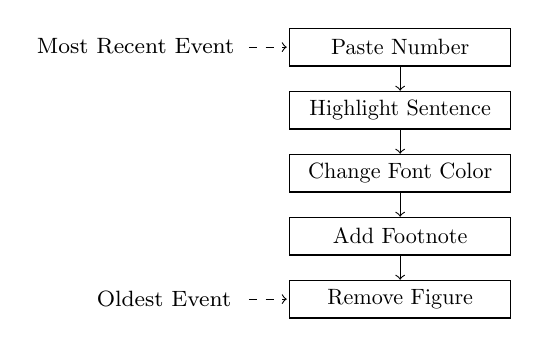
\begin{tikzpicture}[
  scale=.8,
  stacknode/.style={rectangle, draw, minimum width=1.5cm, minimum height=0.6cm, minimum width=3.5cm, text centered,scale=.8},
  dashedarrow/.style={->, dashed}
]

% Stack nodes
\node[stacknode] (top) at (0, 0) {Paste Number};
\node[stacknode] (node1) at (0, -1) {Highlight Sentence};
\node[stacknode] (node2) at (0, -2) {Change Font Color};
\node[stacknode] (node3) at (0, -3) {Add Footnote};
\node[stacknode] (bottom) at (0, -4) {Remove Figure};

% Arrows
\draw[->] (top.south) -- (node1.north);
\draw[->] (node1.south) -- (node2.north);
\draw[->] (node2.south) -- (node3.north);
\draw[->] (node3.south) -- (bottom.north);

% Line of text and dashed arrow
\draw[dashedarrow] (-2.4, 0) -- (-1.8, 0);
\node[align=center] at (-4.2, 0.025) {\footnotesize{}Most Recent Event};

\draw[dashedarrow] (-2.4, -4) -- (-1.8, -4);
\node[align=center] at (-3.75, -4) {\footnotesize{}Oldest Event};

\end{tikzpicture}
\end{center}
\caption{Example of ``Undo'' Event Stack in Text-Editing Program}
\label{fig:stackundo}
\end{figure}

\myexample{As a very basic example of working the \ttt{Stack} data structure, let's design the \ttt{int sumOdds(Stack<Integer> S)} method that, when given a stack of integers~$S$, returns the sum of all odd integer elements.}
Remember that we cannot access arbitrary elements of the stack.
So, for now, all we can do is traverse over the stack using a while loop until it has no elements remaining.
That is, while the stack is non-empty, pop the top-most element, examine if it is odd and, if so, add it to our running total.
We present the following example to demonstrate some of the methods that Java's \ttt{Stack} class provides.\footnote{By providing a \ttt{List} to the \ttt{Stack} constructor, i.e., \ttt{new Stack<>(List.of(...))}, we do not need to write repeated calls to \ttt{push} on the stack object.}

\enlargethispage{2\baselineskip}
\begin{lstlisting}[language=MyJava]
import static Assertions.assertAll;
import static Assertions.assertEquals;
import java.util.Stack;

class StackSumOddsTester {

  @Test
  void testSumOdds() {
    Stack<Integer> S1 = new Stack<>();
    Stack<Integer> S2 = new Stack<>(List.of(5, 12, 13, 24, 91, 108));
    Stack<Integer> S3 = new Stack<>(List.of(7, 5));
    Stack<Integer> S4 = new Stack<>(List.of(2, 100, 42));
    assertAll(
      () -> assertEquals(0, sumOdds(S1));
      () -> assertEquals(109, sumOdds(S2));
      () -> assertEquals(13, sumOdds(S3));
      () -> assertEquals(0, sumOdds(S4)));
  }
}
\end{lstlisting}

\begin{lstlisting}[language=MyJava]
import java.util.Stack;

class StackSumOdds {

  /**
   * Sums the odd numbers in a given stack of integers.
   * @param S - stack of integers.
   * @return sum of odd integers.
   */
  static int sumOdds(Stack<Integer> S) {
    int sum = 0;
    while (!S.isEmpty()) {
      int top = S.pop();
      sum += top % 2 != 0 ? top : 0;
    }
    return sum;
  }
}
\end{lstlisting}


\subsubsection*{\ttt{Queue} Interface}
Imagine you are in line at an amusement park for the most intense roller coaster in the world. 
Another, perhaps more generic term for a ``line'' is a \emph{queue}\index{queue}.
In this metaphor, riders enqueue the line at the back and board the roller coaster (and hence dequeue from the line) at the front. 

What we have described is a practical example of the queue data structure. 
In a queue, elements are enqueued, or inserted, onto the back of the queue, and are dequeued, or removed, from the front. 
Queues operate on the principle of first-in-first-out, or FIFO\index{first-in-first-out}. 
The implementation of a queue data structure may contain different names for their operations, but at their core should contain operations for inserting an element to the back of the queue (e.g., \textsc{enqueue}\index{enqueue}) and removing an element from the front of the queue (e.g., \textsc{dequeue}\index{dequeue}). 

Like the operations of a stack, \textsc{enqueue} and \textsc{dequeue} are also constant-time, since we store references to the front and rear elements of a queue. 
Queues, consequently, share similar drawbacks to stacks in that elements are not randomly accessible, i.e., we only know what exists at the front and rear of a queue instantaneously. 
Figure~\ref{fig:printerqueue} demonstrates the task queue of a printer, which has a sequence of files to print, one after another.

\begin{figure}[ht]
\begin{center}
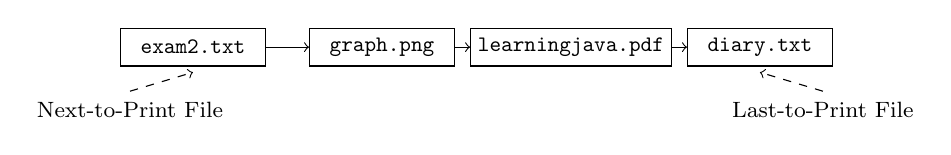
\begin{tikzpicture}[
    scale=.8,
  queuenode/.style={rectangle, draw, minimum width=1.5cm, minimum height=0.6cm, minimum width=2.3cm, text centered,scale=.8},
  dashedarrow/.style={->, dashed}
]

% Queue nodes
\node[queuenode] (front) at (0, 0) {\texttt{exam2.txt}};
\node[queuenode] (node1) at (3, 0) {\texttt{graph.png}};
\node[queuenode] (node2) at (6, 0) {\texttt{learningjava.pdf}};
\node[queuenode] (node3) at (9, 0) {\texttt{diary.txt}};

% Arrows
\draw[->] (front.east) -- (node1.west);
\draw[->] (node1.east) -- (node2.west);
\draw[->] (node2.east) -- (node3.west);

\draw[dashedarrow] (-1, -.7) -- (0, -.4);
\node[align=center] at (-1, -1) {\footnotesize{}Next-to-Print File};

\draw[dashedarrow] (10, -.7) -- (9, -.4);
\node[align=center] at (10, -1) {\footnotesize{}Last-to-Print File};

\end{tikzpicture}
\end{center}
\caption{Example of Printer Task Queue}
\label{fig:printerqueue}
\end{figure}

Unfortunately and inconveniently, there is no \ttt{Queue} class in Java. 
Instead, \texttt{Queue} is an \emph{interface}\index{interface} that other classes implement whose structure models the behavior of a queue. 
To create a first-in-first-out queue data structure, we initialize a variable to be a \texttt{Queue}, then instantiate it as a \texttt{LinkedList}. 
Thankfully, the \texttt{LinkedList} class contains all the relevant methods for operating a FIFO-based queue.

\begin{verbnobox}[\small]
Queue<Integer> q = new LinkedList<>();
\end{verbnobox}

Treating \texttt{q} as a queue rather than a linked list is easy thanks to the methods supplied by the \texttt{LinkedList}\index{\ttt{LinkedList}} implementation. 
Figure~\ref{fig:queues} shows some of these handy methods. 

\begin{figure}[tp]
  \small
  \begin{tcolorbox}[title=Java Queue]
    A \emph{Queue}\index{queue}\index{\ttt{Queue}} is a first-in-first-out (FIFO) sequential data structure where each element is linked to the element immediately after.
    \vspace{2ex}
  \begin{description}
    \item [\ttt{Queue<$T$> $Q=$ new LinkedList<>$()$}] creates a \ttt{Queue} of type $T$, named $Q$.
     \item [\ttt{void $Q$.addLast$(e)$}] adds $e$ to the end of $Q$, placing it at the end of the queue structure.
     \item [\ttt{$T$ $Q$.poll$()$}] returns and removes the element from the front of the queue.
     \item [\ttt{$T$ $Q$.peek$()$}] returns the front-most element in the queue.
    \item [\ttt{int $Q$.size$()$}] returns the number of logical elements in the queue.
  \end{description}
\end{tcolorbox}
  \caption{Useful \ttt{Queue}-based Methods.}
  \label{fig:queues}
\end{figure}

\subsubsection*{\ttt{PriorityQueue} Class}
\begin{figure}[tp]
  \small
  \begin{tcolorbox}[title=Java PriorityQueue]
    A \emph{Priority queue}\index{priority queue} is a rank/score-based data structure wherein the ordering of elements is determined by either their natural ordering or a \ttt{Comparator}.
    \vspace{2ex}
  \begin{description}
    \item [\ttt{PriorityQueue<$T$> $PQ=$ new PriorityQueue<>$(c)$}] creates a \ttt{PriorityQueue} of type $T$, named $PQ$, with a \ttt{Comparator} $c$ that is used to compare objects of type $T$ within the priority queue.
     \item [\ttt{void $PQ$.add$(e)$}] inserts $e$ into $PQ$, whose position in the priority queue depends on the currently-existing elements.
     \item [\ttt{$T$ $PQ$.poll$()$}] returns and removes the element with the highest priority.
     \item [\ttt{$T$ $PQ$.peek$()$}] returns the element with the highest priority.
    \item [\ttt{int $PQ$.size$()$}] returns the number of logical elements in the priority queue.
  \end{description}
\end{tcolorbox}
  \caption{Useful \ttt{PriorityQueue}-based Methods.}
  \label{fig:priorityqueues}
\end{figure}

\emph{Priority queues}\index{priority queues} are the final sequential data structure that we will discuss from the Collections API\@. 
Though, placing priority queues in this section feels a bit disingenuous because, while priority queues have an ordering in their underlying data structure, saying that elements correspond to an index is a misnomer. 
Priority queues, as the name suggests, rank items in the queue by a score called the \emph{priority}\index{priority}. 
Elements with the highest priority are at the ``front'' of the priority queue. 
Inserting elements into a priority queue potentially alters the positioning of preexisting elements.

Priority queues base priority on one of two contributing factors: either the \emph{natural ordering}\index{natural ordering} of elements, or a \emph{comparator object}\index{comparator object}. 
The natural ordering of elements is straightforward: natural ordering for numbers is their standard numeric ordering from least to greatest. 
For strings, the natural ordering is their lexicographical ordering. 
Natural ordering, however, are not as interesting as comparators, which we will now discuss.

A \emph{comparator}\index{comparator} is a way of comparing two arbitrary ``things.'' 
Whether these ``things'' are numbers (i.e., the wrapper classes), strings, or another kind of object, we can define custom ways of comparing \emph{any} non-primitive datatype.

\myexample{Let's design a \ttt{Comparator}\index{\ttt{Comparator}} for prioritizing strings that start with the lowercase letter \ttt{\q{p}\q{}}}.
Comparators are constructed like all other objects via \ttt{new}, but something interesting about their implementation is that we must specify \emph{how} to compare two objects. 
Therefore, when we create a new instance of \ttt{Comparator}, we must also override its \ttt{compare} method. 
The \ttt{compare} method's signature varies based on the parameterized type provided to the comparator, but since we want to compare strings, we should declare it as follows:

\begin{lstlisting}[language=MyJava]
import java.util.Comparator;
import java.util.PriorityQueue;

class PriorityQueueByP {

  /**
   * Returns a priority queue that prioritizes strings 
   * that start with `p'.
   * @return priority queue instance.
   */
  static PriorityQueue<String> priorityByP() {
    Comparator<String> c = new Comparator<>(
      @Override
      public int compare(String s1, String s2) { /* TODO. */ }
    );
  }
}
\end{lstlisting}

We now must describe how we want to compare~\ttt{s1} and~\ttt{s2} to achieve our goal.
Strangely enough, if we want to say that~\ttt{s1} has a higher priority than~\ttt{s2}, we must return a negative value, similar to the natural ordering of strings (this idea extends to any type we wish to compare, however). 
Fortunately, this is not as strange once we understand \emph{why} the negative value is required. 
A value of~$-1$ comes before~$1$ when placing numbers in ascending order. 
Consequently, when comparing an arbitrary value~$t_1$ against~$t_2$, to say that~$t_1$ comes before~$t_2$, we return a negative integer. Conversely, to say that~$t_1$ comes after~$t_2$, we return a positive number.

Let's perform a case analysis on the input strings. 
If both provided strings are non-empty, we retrieve their first character. 
If both start with \ttt{\q{}p\q{}}, then their ordering depends on a standard lexicographical comparison of the rest of the strings. 
If the first character of~$s_1$ is \ttt{\q{}p\q{}}, however, we return~$-1$ to designate that~$s_1$ has a higher priority than~$s_2$. 
Conversely, if~$s_2$ starts with \ttt{\q{}p\q{}}, then we return~$1$ to designate the opposite. 
If neither start with~$p$, then again we perform a lexicographical comparison on the entire strings. 
Algorithm~\ref{alg:pseudocodepriority} displays the pseudocode for the comparator, but as we will see, we can translate this, verbatim, into Java syntax. 
The last line of \ttt{priorityByP} instantiates a new \ttt{PriorityQueue}\index{\ttt{PriorityQueue}} whose constructor receives the \ttt{Comparator}\index{\ttt{Comparator}} that we just designed. 

\begin{algorithm}[H]
\begin{algorithmic}
\Procedure{Compare}{$s_1$, $s_2$}
    \If {$s_1$ \textbf{and} $s_2$ are non-empty}
        \State $c_1 \gets \textbf{First}(s_1)$
        \State $c_2 \gets \textbf{First}(s_2)$
        \If {$c_1$ is `p' \textbf{and} $c_2$ is `p'}
            \State $xs_1 \gets s_1$\emph{.substring(1)}
            \State $xs_2 \gets s_2$\emph{.substring(1)}
            \State \Return $xs_1$\emph{.compareTo}$(xs_2)$
        \ElsIf {$c_1$ is `p'}
            \State \Return $-1$
        \ElsIf {$c_2$ is `p'}
            \State \Return $1$
        \Else
            \State \Return $s_1$\emph{.compareTo}$(s_2)$
        \EndIf
    \Else
        \State \Return $s_1$\emph{.compareTo}$(s_2)$
    \EndIf
\EndProcedure
\end{algorithmic}
\caption{Pseudocode for Comparing Two Strings For `p' Priority}
\label{alg:pseudocodepriority}
\end{algorithm}

\begin{lstlisting}[language=MyJava]
import java.util.Comparator;
import java.util.PriorityQueue;

class PriorityQueueByP {

  static PriorityQueue<String> priorityByP() {
    Comparator<String> c = new Comparator<>() {
      @Override
      public int compare(String s1, String s2) {
        if (!s1.isEmpty() && !s2.isEmpty()) {
          char c1 = s1.charAt(0);
          char c2 = s2.charAt(0);
          if (c1 == 'p' && c2 == 'p') {
            return s1.substring(1).compareTo(s2.substring(1));
          } else if (c1 == 'p') {
            return -1;
          } else if (c2 == 'p') {
            return 1;
          } else {
            return s1.compareTo(s2);
          }
        } else {
          return s1.compareTo(s2);
        }
      }
    };
    return new PriorityQueue<String>(c);
  }
}
\end{lstlisting}

Let us add a few elements to a priority queue with our custom comparator to exemplify the idea. To add elements, we use \ttt{.add}, and to remove the element with the highest priority, we invoke \ttt{.poll}.

\enlargethispage{-2\baselineskip}
\begin{lstlisting}[language=MyJava]
import java.util.Comparator;
import java.util.PriorityQueue;

class PriorityQueueByP {

  static PriorityQueue<String> priorityByP() { /* Code hidden. */ }

  public static void main(String[] args) {
    PriorityQueue<String> pq1 = priorityByP();
    // Add a few values.
    pq1.add("pool"); pq1.add("peek"); pq1.add("hello"); pq1.add("barks");
    pq1.add("park"); pq1.add("pecking"); pq1.add("shrub");

    // Poll each from the queue and print them out.
    while (!pq1.isEmpty()) { System.out.println(pq1.poll()); }
  }
}
\end{lstlisting}

The output is as follows:

\begin{verbnobox}[\small]
park
pecking
peek
pool
barks
hello
shrub
\end{verbnobox}

With the provided comparator, \ttt{park} has the highest priority because it starts with \ttt{\q{}p\q{}} and has a substring that comes before the rest of those strings starting with \ttt{\q{}p\q{}}. 
The strings \ttt{pecking}, \ttt{peek}, and \ttt{pool} come next for similar reasons. 
Finally, none of the strings \ttt{barks}, \ttt{hello}, and \ttt{shrub} start with \ttt{\q{}p\q{}}, so we compare based on the strings themselves. 
The underlying implementation of \emph{how} the priority queue works and enforces ordering is beyond the scope of this textbook. 
Such details are reserved for a textbook or course on advanced data structures, which follows the course designed for the audience of this text.

\subsection{Set-Based Data Structures}
\emph{Sets} are unordered collections of non-duplicate elements. 
Does this definition sound familiar? 
It should; it perfectly mirrors the mathematical definition of a set. 
Java has a few nuances to its definition of sets that we will now see. 
We consider these data structures \emph{set-based} since they all rely on the ``no-duplicate'' philosophy.

\subsubsection*{\ttt{Set} Interface}
A \emph{Set}\index{set}\index{\ttt{Set}} in Java is an interface rather than a class. 
This is because Java has a hierarchy for differing implementations of sets. 
We will discuss three such implementations: \emph{HashSet}, \emph{TreeSet}, and \emph{LinkedHashSet}. 
While all three disallow duplicate elements, the latter two impose an ordering on their elements, which goes against the standard mathematical definition, but for practical reasons.

\subsubsection*{\ttt{HashSet} Class}
In the implementation of a \ttt{HashSet}\index{hash set}\index{\ttt{HashSet}}, the existence of objects in the set is determined by the \ttt{hashCode()} method of the objects, which computes their hash codes. 
These hash codes are used to decide in which `bucket' within the hash table an object should be placed. 
It's important, though, to note that hash codes are not used for comparing the equality of the content of objects. 
Unlike the \ttt{==} operator, which checks if two references point to the same object in memory, the respective \ttt{equals()} method is used to compare the actual content of the objects. 
When adding an object to a \ttt{HashSet}, if the hash code of the object matches the hash code of any existing object in the corresponding bucket, the \ttt{equals()} method is then used to check for actual content equality to ensure that no duplicate objects (in terms of content) are added to the set. 
In other words, two objects that are equal in terms of \ttt{equals()} must have the same hashcode, but the converse is not necessarily true. 
Anything more than these details goes beyond the scope of this textbook, but we will provide a small synopsis of hashable data structures.

A hashable data structure is most often designed as a hash table, which is similar to an array, where elements are stored. 
Hashable data structures are known for their fast lookup times, thanks to a \emph{hash function}\index{hash function}: a mathematical function used to compute the location to store a value in a hash table. 
Consider a hash function~$H(v)$, whose range is the set of integers~$[0, n)$, where~$n$ is the number of elements of the hash table. 
Running~$v$ (which is an arbitrary argument) through the hash function~$H$ returns an index of the hash table. 
Evaluating~$H$ is, in optimal conditions, a constant-time algorithm, hence determining value existence in a hash table also runs in constant-time. 
This begs the question of what happens if there exists an output of~$H$ such that~$H(v') = H(v)$, but $v' \neq v$. 
In subsequent computer science courses, students learn how to resolve \emph{hash collisions}\index{hash collisions} through techniques such as linear and quadratic probling, as well as chaining.\footnote{In Chapter~\ref{chapter-classes}, we will implement a simple hash table that uses chaining to resolve hash collisions.}
%The previous paragraph briefly discussed this through the `buckets' analogy and \ttt{equals}, but we will ignore such complexities and use hashable data structures at face value.  

Use hashsets when you do not care about element ordering or ``position'' in the set, and want to ensure no duplicates exist.
\begin{figure}[tp]
  \small
  \begin{tcolorbox}[title=Java Sets]
    A \emph{Set}\index{set}\index{\ttt{Set}} is a data structure of non-duplicate elements, with \ttt{HashSet} being the most common implementation/usage of sets.
    \vspace{2ex}
  \begin{description}
    \item [\ttt{Set<$T$> $S=$ new HashSet<>$()$}] creates a \ttt{HashSet} of type $T$, named $S$.
     \item [\ttt{boolean $S$.contains$(e)$}] returns whether or not $e$ is in the set $S$.
     \item [\ttt{boolean $S$.add$(e)$}] adds $e$ to the set $S$ only if it is not present. If $e$ is not in $S$, it returns \ttt{false}; otherwise, it returns \ttt{true}.
     \item [\ttt{boolean $S$.remove$(e)$}] removes $e$ from the set $S$ only if it is present. If $e$ is not in $S$, it returns \ttt{false}; otherwise, it returns \ttt{true}.
    \item [\ttt{int $S$.size$()$}] returns the number of logical elements in the set.
  \end{description}
\end{tcolorbox}
  \caption{Useful \ttt{Sets}-based Methods.}
  \label{fig:hashsets}
\end{figure}

\subsubsection*{\ttt{TreeSet} Class}
A \emph{TreeSet}\index{tree set}\index{\ttt{TreeSet}} is a set with determined order, either by the natural ordering of the elements or one defined by a \ttt{Comparator}, similar to a priority queue. 
All methods in a \ttt{Set} are, definitionally, implemented by a \ttt{TreeSet}.

\subsubsection*{\ttt{LinkedHashSet} Class}
A \emph{LinkedHashSet}\index{linked hash set}\index{\ttt{LinkedHashSet}} is a set with an ordering based on the insertion order of the elements. 
All methods in a \ttt{Set} are, definitionally, implemented by a \ttt{LinkedHashSet}.

\myexample{The canonical usage of a set is to remove duplicates from a list.} 
Indeed, let's design the \ttt{removeDuplicatesList} method that receives a list of integers and returns a new list without any duplicates. 
We will add a postcondition requirement that the output order of the integers must match the input order. 
To solve this problem, we will create an auxiliary linked hash set data structure, add all elements from the list into the set, then add those values from the set to a new list. 
When adding a value into a set, if it already exists, it is not re-added.

%\enlargethispage{4\baselineskip}
\begin{lstlisting}[language=MyJava]
import static Assertions.assertAll;
import static Assertions.assertEquals;

import java.util.List;

class RemoveDuplicatesListTester {

  @Test
  void testRemoveDuplicatesList() {
    assertAll(
      () -> assertEquals(List.of(), 
                         removeDuplicatesList(List.of())),
      () -> assertEquals(List.of(1, 2, 3, 4), 
                         removeDuplicatesList(List.of(1, 1, 2, 2, 3, 3, 4, 4))),
      () -> assertEquals(List.of(3, 1, 4), 
                         removeDuplicatesList(List.of(3, 1, 1, 3, 4, 4, 3, 4))));
  }
}
\end{lstlisting}

\enlargethispage{3\baselineskip}
\begin{lstlisting}[language=MyJava]
import java.util.List;
import java.util.ArrayList;
import java.util.Set;
import java.util.LinkedHashSet;

class RemoveDuplicatesList {

  /**
   * Removes duplicates from a list of integers.
   * @param ls - list of integers.
   * @return new list without duplicates.
   */
  static List<Integer> removeDuplicatesList(List<Integer> ls) {
    List<Integer> newLs = new ArrayList<>();
    Set<Integer> set = new LinkedHashSet<>();
    for (int x : ls) { set.add(x); }
    for (int x : s) { newLs.add(x); }
    return newLs;
  }
}
\end{lstlisting}

\myexample{Suppose we want to find all common elements shared between two linked lists of elements, which are unordered.} 
Let's design the \ttt{commonValues} method that, when given two linked lists of integers, returns a sorted-ordered list of the values that occur in both lists. 
We should not count values twice, e.g., if \ttt{2} occurs twice in the first list, then the resulting output list should only contain one occurrence of \ttt{2}. 
Let's take advantage of a tree set to store the common values in order, and then add those values to a new linked list.

%\enlargethispage{2\baselineskip}
\begin{lstlisting}[language=MyJava]
import static Assertions.assertAll;
import static Assertions.assertEquals;

import java.util.List;
import java.util.LinkedList;
import java.util.Set;
import java.util.TreeSet;

class CommonValuesTester {

  @Test
  void testCommonValues() {
    assertAll(
      () -> assertEquals(List.of(), 
                         commonValues(List.of(),
                                      List.of(5, 4, 3, 2, 1))),
      () -> assertEquals(List.of(), 
                         commonValues(List.of(10, 20, 30, 40, 50),
                                      List.of(5, 4, 3, 2, 1))),
      () -> assertEquals(List.of(1, 3, 4), 
                         commonValues(List.of(2, 4, 1, 3, 5, 6),
                                      List.of(1, 4, 3, 10, 20))),
      () -> assertEquals(List.of(-2, 0, 2), 
                         commonValues(List.of(2, -2, 0, 0, -2, 2),
                                      List.of(-2, 2, 0))));
  }
}
\end{lstlisting}

\enlargethispage{1\baselineskip}
\begin{lstlisting}[language=MyJava]
import java.util.List;
import java.util.LinkedList;
import java.util.Set;
import java.util.TreeSet;

class CommonValuesTester {

  /**
   * Finds all common values between two linked lists of integers.
   * @param ls1 - first linked list.
   * @param ls2 - second linked list.
   * @return list of (distinct) common values.
   */
  static List<Integer> commonValues(LinkedList<Integer> ls1, LinkedList<Integer> ls2) {
    Set<Integer> set = new TreeSet<>();
    for (int x : ls1) {
      if (ls2.contains(x)) { set.add(x); }
    }
    List<Integer> newLs = new LinkedList<>();
    newLs.addAll(set);
    return newLs;
  }
}
\end{lstlisting}

\myexample{We are given an array of numbers from~$1$ to~$n$, where one number is missing and one is duplicated. 
Let's design the \ttt{findDupMissing} method that returns an array of two elements: the first of which is the missing number and the second of which is the duplicate value. 
It makes sense to use a \ttt{TreeSet} since, that way, we can store the numbers in order and find out which one is omitted through one traversal, and find the only duplicate.}


\begin{lstlisting}[language=MyJava]
import static Assertions.assertAll;
import static Assertions.assertArrayEquals;

class FindDupMissingTester {

  @Test
  void testFindDupMissing() {
    assertAll(
      () -> assertArrayEquals(new int[]{2, 3}, 
                              findDupMissing(new int[]{1, 3, 3, 4})),
      () -> assertArrayEquals(new int[]{5, 1}, 
                              findDupMissing(new int[]{8, 1, 4, 1, 3, 2, 6, 7})),
      () -> assertArrayEquals(new int[]{6, 7}, 
                              findDupMissing(new int[]{3, 2, 7, 7, 4, 5, 1})));
  }
}
\end{lstlisting}

\enlargethispage{1\baselineskip}
\begin{lstlisting}[language=MyJava]
import java.util.Set;
import java.util.TreeSet;

class FindDupMissing {

  /**
   * Finds a duplicate number and a missing number from 
   * an array of numbers within a specific interval.
   * @param A - array of integers where each number is in [1, n],
   *            with one missing and one duplicate.
   * @return two-element array where [0] is the missing number
   *         and [1] is the duplicate number.
   */
  static int[] findDupMissing(int[] A) {
    Set<Integer> set = new TreeSet<>();
    int[] res = new int[2];
    // Add the values to the set and find the duplicate one.
    for (int x : A) {
      if (set.contains(x)) { res[1] = x; } 
      else { set.add(x); }
    }

    // Now find the missing number.
    int prev = 0;
    for (int x : set) {
      if (x != prev + 1) {
        res[0] = prev + 1;
        break;
      } else {
        prev = x;
      }
    }
    return res;
  }
}
\end{lstlisting}

\subsection{Dictionary-Based Data Structures}
Dictionaries map elements from one type~$K$ to elements of another type~$V$. The types~$K$ and~$V$ do not necessarily need to be distinct. 

\subsubsection*{\ttt{Map} Interface}
Java has an interface called \ttt{Map}\index{map}\index{\ttt{Map}} rather than a class because, like sets, there is a hierarchy for differing implementations of maps. 
We will discuss three: \emph{HashMap}, \emph{TreeMap}, and \emph{LinkedHashMap}.
Maps contain keys and values; the keys are mapped to values in the map. 
A key/value pairing is called an \emph{entry}\index{entry}, or an \emph{association}\index{association}.
Maps cannot contain duplicate keys, because it would be ambiguous to have two identical keys mapping to different values.

\subsubsection*{\ttt{HashMap} Class}
\emph{HashMaps}\index{hash map}\index{\ttt{HashMap}} base existence of keys in the map by their hashcode and a hash table, identical to a hash set. 
For a greater detail of how hashable data structures work, please refer to the previous subsection.

\begin{figure}[tp]
  \small
  \begin{tcolorbox}[title=Java Maps]
    A \emph{Map}\index{map} is a dictionary-based data structure wherein we map \emph{keys} to \emph{values}, with \ttt{HashMap} being the most common implementation/usage of maps.
    \vspace{2ex}
  \begin{description}
    \item [\ttt{Map<$K, V$> $M=$ new HashMap<>()}] creates a \ttt{HashMap} named $M$ whose keys are of type $K$ and whose values are of type $V$. Namely, the keys map to the values.
     \item [\ttt{$M$.containsKey$(k)$}] returns whether or not $k$ is a key in the map $M$.
     \item [\ttt{void $M$.put$(k, v)$}] maps the key $k$ to the value $v$ in $M$.
     \item [\ttt{$V$ $M$.get$(k)$}] returns the value associated with $k$ in $M$, or \ttt{null} if $k$ has no association.
     \item [\ttt{$V$ $M$.getOrDefault($k$, $x$)}] returns the value associated with $k$ in $M$, or $x$ if $k$ does not have an association.
    \item [\ttt{int $M$.size$()$}] returns the number of logical elements in the set.
    \item [\ttt{Set<$K$> keySet$()$}] returns a set of the keys in the map.
  \end{description}
\end{tcolorbox}
  \caption{Useful \ttt{Map}-based Methods.}
  \label{fig:hashmap}
\end{figure}

\subsubsection*{\ttt{TreeMap} Class}
A \emph{TreeMap}\index{tree map}\index{\ttt{TreeMap}} is a map with a determined order, either by a natural ordering of the keys or that defined by a comparator. 
All methods in \texttt{Map} are, definitionally, implemented by a \texttt{TreeMap}.

\subsubsection*{\ttt{LinkedHashMap} Class}
A \emph{LinkedHashMap}\index{linked hash map}\index{\ttt{LinkedHashMap}} is a map with an ordering based on the insertion order of the key/value pairs. 
All methods in a \ttt{Map} are, definitionally, implemented by a \ttt{LinkedHashMap}.

\myexample{Perhaps one of the most common use cases for a dictionary-based data structure is to compute the frequency, or count, of some values.} 
Suppose we want to design the \ttt{mode} method that, when given a list of integers, returns the mode(s), i.e., the most-frequent value(s). 
We can use a map to keep track of the numbers seen so far, which are the keys, and their respective frequencies being the values. 
Because a list of numbers may have multiple modes, we will need to use a three-step algorithm:

%\enlargethispage{4\baselineskip}
\begin{enumerate}
  \item Compute the frequencies of each number.
  \item Find the highest frequency.
  \item Find all numbers that match this frequency.
\end{enumerate}

Traversing over a map is straightforward: we obtain a \emph{key set}\index{key set}, which is a set of the keys in a map, and each corresponding value is retrieved via one call to the \ttt{.get} method.

\begin{lstlisting}[language=MyJava]
import static Assertions.assertAll;
import static Assertions.assertEquals;

import java.util.List;
import java.util.Set;

class ComputeModeTester {

  @Test
  void testMode() {
    assertAll(
      () -> assertEquals(Set.of(), mode(List.of())),  
      () -> assertEquals(Set.of(3), mode(List.of(4, 5, 2, 3, 3, 4, 3))),
      () -> assertEquals(Set.of(2, 3), mode(List.of(2, 3, 2, 3, 3, 2))),
      () -> assertEquals(Set.of(2), mode(List.of(2, 2, 2, 2, 2, 2, 2))));
  }
}
\end{lstlisting}

\enlargethispage{-6\baselineskip}
\begin{lstlisting}[language=MyJava]
import java.util.HashMap;
import java.util.HashSet;
import java.util.List;
import java.util.Map;
import java.util.Set;

class ComputeMode {

  /**
   * Computes the mode of a list of numbers, which is the most-frequent value(s).
   * @param ls - list of numbers.
   * @return set of mode values, if they exist.
   */
  static Set<Integer> mode(List<Integer> ls) {
    if (ls.isEmpty()) { return new HashSet<>(); } 
    else {
      // First, compute the frequencies.
      Map<Integer, Integer> frequencies = new HashMap<>();
      for (int v : ls) {
        if (!frequencies.containsKey(v)) {
          frequencies.put(v, 1);
        } else {
          frequencies.put(v, frequencies.get(v) + 1);
        }
      } 

      // Find the highest frequency.
      int highestFreq = -1;
      for (int k : frequencies.keySet()) {
        highestFreq = Math.max(highestFreq, frequencies.get(k));
      }

      // Now, find the values that match that frequency.
      return frequencies.keySet()
                        .stream()
                        .filter(k -> frequencies.get(k) == highestFreq)
                        .collect(Collectors.toSet());
    }
  }
}
\end{lstlisting}

\myexample{Let's design the \ttt{sharesFirstChar} method that, when given an array of strings, returns a \ttt{Map<Character, Set<String>{>}} such that each alphabetized character maps to a set of alphabetized strings that start with that character.} 
We will further assume a case-insensitive mapping. 
Consider the following input and output example:

\begin{verbnobox}[\small]
sharesFirstChar(["she", "sells", "sea", "shells", "by", "the", "sea"])
  => [<'b' : {"by"}>, 
      <'s' : {"sea", "sells", "she", "shells"}>
      <'t' : {"the"}>]
\end{verbnobox}

Because we want both the sets and maps to be alphabetized, the use of a \ttt{TreeSet} and \ttt{TreeMap} is appropriate. 
So, we will first traverse over the input list and instantiate a map whose keys are the first letters of each word, and whose value is a new instance of a \ttt{TreeSet}. 
We then populate the sets via a second traversal over the list.

\begin{lstlisting}[language=MyJava]
import static Assertions.assertAll;
import static Assertions.assertEquals;

import java.util.List;
import java.util.Map;
import java.util.Set;
import java.util.TreeMap;

class ShareFirstCharacterTester {
  
  @Test
  void testShareFirstChar() {
    Map<Character, Set<String>> exp1 = new TreeMap<>();
    assertEquals(exp1, shareFirstChar(List.of()));

    Map<Character, Set<String>> exp2 = new TreeMap<>();
    exp2.put('b', new TreeSet<>());
    exp2.put('s', new TreeSet<>());
    exp2.put('t', new TreeSet<>());
    exp2.get('s').addAll(Set.of("she", "sells", "sea", "shells"));
    exp2.get('t').addAll(Set.of("the"));
    exp2.get('b').addAll(Set.of("by"));
    assertEquals(exp2, 
                 shareFirstChar(List.of("she", "sells", "sea", "shells", 
                                        "by", "the", "sea")));
  }
}
\end{lstlisting}

%\enlargethispage{4\baselineskip}
\begin{lstlisting}[language=MyJava]
import java.util.HashMap;
import java.util.List;
import java.util.Map;
import java.util.Set;
import java.util.TreeSet;

class ShareFirstCharacter {

  /**
   * Returns a map whose keys are the first characters of the strings
   * and whose values are sets of strings that start with that character.
   * @param ls - list of strings.
   * @return map of sets of strings.
   */
  static Map<Character, Set<String>> shareFirstChar(List<String> ls) {
    Map<Character, Set<String>> M = new HashMap<>();
    // Populate the map with the initial TreeSets.
    for (String s : ls) {
      char lc = Character.toLowerCase(s.charAt(0));
      if (!M.containsKey(lc)) {
        M.put(lc, new TreeSet<>());
      }
    }

    // Add the strings to each set.
    for (String s : ls) {
      M.get(Character.toLowerCase(s.charAt(0))).add(s);
    }
    return M;
  }
}
\end{lstlisting}

\myexample{Let's design the \ttt{firstUniqueDigit} method that, when given a string, returns the first non-repeated digit.} 
If there is no non-repeated digit, then return the empty string. 
Because we care about the insertion order, we should use a \ttt{LinkedHashMap} whose keys are characters in the string and whose values are frequency counts. 
The idea is to count the frequency of each (digit) character, then traverse over the linked map and find the first key whose (value) frequency is one. 
Because we now understand how to combine \ttt{get} and \ttt{put} to insert and increment frequency counts, we will instead opt to use \ttt{getOrDefault}, which removes the need for the conditional.\footnote{This problem is similar to one created by \ttt{frew@mclean.com} on \ttt{codingbat.com}. Thanks!}

\enlargethispage{-2\baselineskip}
\begin{lstlisting}[language=MyJava]
import static Assertions.assertAll;
import static Assertions.assertEquals;

class FirstUniqueDigitTester {

  @Test
  void testFirstUniqueDigit() {
    assertAll(
      () -> assertEquals("3", firstUniqueDigit("1211312121")),
      () -> assertEquals("2", firstUniqueDigit("0099828776")),
      () -> assertEquals("", firstUniqueDigit("11223344")));
  }
}
\end{lstlisting}

%\enlargethispage{2\baselineskip}
\begin{lstlisting}[language=MyJava]
import java.util.HashMap;
import java.util.Map;

class FirstUniqueDigit {

  /**
   * Returns the first unique digit in a string, as a string. 
   * If there is no unique digit, then the empty string is returned.
   * @param s - string.
   * @return first unique digit as a string.
   */
  static String firstUniqueDigit(String s) {
    Map<Character, Integer> M = new LinkedHashMap<>();
    // Count the frequency of each digit
    for (int i = 0; i < s.length(); i++) {
      String c = s.substring(i, i + 1);
      if (Character.isDigit(c.charAt(0))) {
        M.put(c.charAt(0), M.getOrDefault(c.charAt(0), 0) + 1);
      }
    }

    // Find the first unique letter.
    for (char c : M.keySet()) {
      if (M.get(c) == 1) {
        return String.valueOf(c);
      }
    }
    return "";
  }
}
\end{lstlisting}

\myexample{One final example that we will consider is the \ttt{nthMostFrequentChar} method that, when given a string~$s$ and an integer~$n$, returns the~$n^\text{th}$ most frequent character in the string, or \ttt{null} if there is no such character.} 
If there are multiple characters that share the same position, we return the first one in terms of lexicographical ordering.

For example, consider the string \ttt{"abbabdcaadaababcdcc"} and~$n=3$. 
The most frequent characters are \ttt{\q{}a\q{}, \q{}b\q{}, \q{}c\q{}}, in that order.
So, the third most frequent character is \ttt{\q{}c\q{}}.

Another example is the string \ttt{"aabbcc"} and~$n=2$. 
The most frequent characters are \ttt{\q{}a\q{}, \q{}b\q{}, \q{}c\q{}}, in that order, but all three characters share a frequency of two, meaning they are all equally frequent. 
In this case, we return the empty string.

A third example is the string \ttt{"aaaabccccc"} and~$n=2$. 
The most frequent characters are \ttt{\q{}c\q{}, \q{}a\q{}, \q{}b\q{}}, in that order.
So, the second most frequent character is \ttt{\q{}a\q{}}.

First, we will count the frequency of each character, then use a \ttt{PriorityQueue} to store the characters in order of their frequency from greatest to least. 
We will then remove the first~$n-1$ characters from the priority queue, and return the first character of the remaining queue. 
This approach may raise some eyebrows, because if the frequency is the value in a map, how can we construct a comparator? 
In other circumstances, one needs access to a particular key to obtain its corresponding value. 
In this instance, though, we can generate the \emph{entry set} for the map of characters to frequencies, which is a set of \ttt{Map.Entry<K, V>} objects, where~$K$ is the key type and~$V$ is the value type. 
Our priority queue comparator receives two such entries~$e$ and~$f$, and performs the following comparison:

\begin{itemize}
  \item If $e_k \neq f_k$, return $f_v - e_v$.
  \item Else, return the lesser of $e_k$ and $f_k$.
\end{itemize}

We know that~$K$ is \ttt{Character} and~$V$ is \ttt{Integer} representing the characters mapped to their frequencies. 
To retrieve the key and value from an \ttt{Map.Entry} object, we use the \ttt{getKey()} and \ttt{getValue()} methods respectively. 
In an effort to keep our code a bit more concise, we will design a private and static helper method to create a \ttt{Comparator} object using the aforementioned criteria.

\begin{lstlisting}[language=MyJava]
import static Assertions.assertAll;
import static Assertions.assertEquals;

class NthMostFrequentCharTester {

  @Test
  void testNthMostFrequentChar() {
    assertAll(
      () -> assertEquals("a", nthMostFrequentChar("abacab", 1)),
      () -> assertEquals("d", nthMostFrequentChar("aaaadddcccccbbee", 3)),
      () -> assertEquals("q", nthMostFrequentChar("ppqrrss", 2)),
      () -> assertEquals(null, nthMostFrequentChar("aabbccdd", 2)));
  }
}
\end{lstlisting}

%\enlargethispage{8\baselineskip}
\begin{lstlisting}[language=MyJava]
import java.util.Comparator;
import java.util.HashMap;
import java.util.Map;
import java.util.PriorityQueue;

class NthMostFrequentChar {

  /**
   * Given a string, returns the nth most 
   * frequent character in that string.
   * @param s - string to examine.
   * @param n - int n >= 0.
   * @return the nth most frequent character as a String or null if nonexistent.
   */
  static String nthMostFrequentChar(String s, int n) {
    // Step 1: compute the frequencies.
    Map<Character, Integer> M = new HashMap<>();
    s.chars().forEach(c -> M.put(c, M.getOrDefault(c, 0))); 

    // Step 2: populate the priority queue with entry objects. Use the comparator.
    PriorityQueue<Map.Entry<Character, Integer>> Q = new PriorityQueue<>(getCmp());
    M.entrySet().forEach(e -> Q.add(e));

    // Step 4: poll n - 1 items from the queue.
    while (!Q.isEmpty()) {
      n--;
      if (n == 0) { return String.valueOf(Q.peek().getKey()); } 
      else { Q.poll(); }
    }
    return null;
  }

  private static Comparator<Entry<Character, Integer>> getCmp() {
    return new Comparator<>() {
      @Override
      public int compare(Map.Entry<Character, Integer> e, 
                         Map.Entry<Character, Integer> f) {
        if (e.getKey() != f.getKey()) {
          return Character.compare(e.getKey(), f.getKey());
        } else {
          return f.getValue() - e.getValue();
        }
      }
    };
  }
}
\end{lstlisting}

\section{Iterators}
We know how to iterate, or traverse, over a simple data structure such as an array. 
The idea is to use a variable for the index and continuously increment it until we reach the upper bound of the array. 
Below is a simple example where we sum the elements of an array.

\begin{verbnobox}[\small]
static int sum(int[] arr) {
  int sum = 0;
  for (int i = 0; i < arr.size; i++) { sum += arr[i]; }
  return sum;
}
\end{verbnobox}

The problem is that not all data structures, as we have undoubtedly seen, are sequential; sets and maps are two examples of non-sequential data structures, so how do we traverse over those? 
One option is the enhanced-for loop, but as we will show later, this approach has its drawbacks, even though its syntax is straightforward. 
Stacks and queues are another example of data structures that are not necessarily sequential. 
\emph{Iterator} objects are one answer to the traversability problem. 
Iterators provide a mechanism for traversing over a data structure. 
Any data structure whose class definition implements \ttt{Iterator} must define at least two methods: \ttt{boolean hasNext} and \ttt{T next}, which determines whether we are at the end of the traversal, and retrieves the next element, respectively. 
Note that \ttt{T}, for the time being, simply means ``any type,'' and is related to type parameterization.
All of the Java collections implement \ttt{Iterator}, and we can retrieve the corresponding \ttt{Iterator} object via the \ttt{.iterator} method. 

Upon retrieving an iterator, we can use a \ttt{while} loop to continuously retrieve elements in the data structure until no more elements remain to be visited. 
The elements of the iterator are generated on-the-fly; only upon calling \ttt{next} is the value truly read from the data structure itself. 
Much like the rest of the Collections API, we must pass the parameterized type to the \ttt{Iterator} initialization, so that it knows what type to substitute for \ttt{T}.

\myexample{Let's use an iterator to traverse over a \ttt{LinkedHashSet}, whose element ordering is determined by their insertion order, meaning that the iterator should produce them in the order that they were inserted.}

%\enlargethispage{5\baselineskip}
\begin{lstlisting}[language=MyJava]
import static Assertions.assertAll;
import static Assertions.assertEquals;

import java.util.Set;
import java.util.LinkedHashSet;
import java.util.Iterator;

class IteratorTester {

  @Test
  void testIterator() {
    Set<Integer> lhs = new LinkedHashSet<>(Set.of(8, 90));
    Iterator<Integer> it = lhs.iterator();
    assertAll(
      () -> assertTrue(it.hasNext());
      () -> assertEquals(8, it.next()),
      () -> assertEquals(90, it.next()),
      () -> assertFalse(it.hasNext()));
  }
} 
\end{lstlisting}

Should we want to traverse over the data again, we need to instantiate another instance of the iterator, because there is no way to reset the ``position'' of an iterator; they are a kind of ``one-time use'' objects.

It should be stated that the enhanced \ttt{for} loop is nearly identical to the job of an \ttt{Iterator}, so a programmer may wonder why not use the former over the latter. 
Inside an enhanced \ttt{for} loop, the data structure in question is immutable, meaning that we cannot add, insert, remove, or change elements. 
On the other hand, iterators allow structural modification. 
We would recommend not altering the data structure while traversing, even if it is permissible by Java, because doing so can produce irksome bugs. 

\myexample{Let's now iterate over the \ttt{LinkedHashSet} using an enhanced \ttt{for} loop.} We can do so by placing the type on the left-hand side of the element declaration. 
Our test subtracts the elements from left-to-right.

\enlargethispage{\baselineskip}
\begin{lstlisting}[language=MyJava]
import static Assertions.assertEquals;

import java.util.Set;
import java.util.LinkedHashSet;

class EnhancedForLoopTester {

  @Test
  void testEnhancedForLoop() {
    Set<Integer> lhs = new LinkedHashSet<>();
    lhs.add(1); lhs.add(2); lhs.add(3); lhs.add(4);
    int diff = 0;
    for (Integer e : lhs) { diff -= e; }
    assertEquals(-10, diff);
  }
}
\end{lstlisting}

\myexample{Not only does the use of an enhanced \ttt{for} loop disallow structural modification, it also does not preserve the order of specific data structures.} 
For example, suppose we have a stack $S=[10, 20, 30, 40, 50]$, where~$50$ is the top of the stack. 
If we want to print each element of~$S$ without iterators or modifying the stack itself, the obvious option is to use an enhanced \ttt{for} loop. 
Unfortunately, this does not go as expected: it prints the elements in the order they are inserted, i.e., first-in-first-out. 
Intuitively, we may expect the program to output the values via last-in-first-out, i.e., $50, 40, 30, 20, 10$. 
What's worse is that its \ttt{Iterator} implementation also makes the glaring mistake. 
The solution proposed by Oracle is to instead use the \ttt{ArrayDeque} class, which is a type of \ttt{Deque} object.\footnote{A \emph{deque}, pronounced as `deck,' is a double-ended queue, meaning we can insert and remove elements from either the front or the rear.}\footnote{See the note listed on Oracle's \ttt{Stack} documentation: \url{https://docs.oracle.com/javase/8/docs/api/java/util/Stack.html}}

%\enlargethispage{-1\baselineskip}
\begin{lstlisting}[language=MyJava]
import java.util.ArrayDeque;
import java.util.Deque;
import java.util.Iterator;
import java.util.List;
import java.util.Stack;

class StackPrinter {

  public static void main(String[] args) {
    Stack<Integer> S = new Stack<>(List.of(10, 20, 30, 40, 50));

    // Enhanced for loop prints them "incorrectly!"
    // An Iterator also has this issue.
    // We get "10, 20, 30, 40, 50" separated by newlines.
    S.forEach(x -> System.out.println(x));

    Deque<Integer> D = new ArrayDeque<>(List.of(10, 20, 30, 40, 50));

    // An ArrayDeque corrects this problem.
    // We correctly get "50, 40, 30, 20, 10" separated by newlines.
    D.forEach(x -> System.out.println(x));
  }
}
\end{lstlisting}

\myexample{The unintuitive nature of the enhanced \ttt{for} loop and certain iterator behavior does not stop with stacks, unfortunately.}
Priority queues are also afflicted as a consequence of their implementation. 
Let's see what happens when we create a priority queue whose comparator prioritizes the string \ttt{"Joshua"} over all strings and makes the string \ttt{"Jack"} have the lowest priority. 
In other words, any occurrence of \ttt{"Joshua"} should come before all other strings in the priority queue, whereas any occurrence of \ttt{"Jack"} should come after all other strings in the priority queue. 
Any strings in between are ordered naturally, i.e., via lexicographical ordering.

\enlargethispage{-6\baselineskip}
\begin{lstlisting}[language=MyJava]
import java.util.List;
import java.util.PriorityQueue;
import java.util.Comparator;

class PriorityQueuePrinting {

  private static PriorityQueue<String> initPriorityQueue() {
    Comparator<String> S = new Comparator<>() {
      @Override
      public int compare(String s1, String s2) {
        // If Joshua comes first or Jack comes last, 
        // then s1 is prioritized.
        if (s1.equals("Joshua") || s2.equals("Jack")) { return -1; } 
        // If Jack comes first or Joshua comes last, 
        // then s2 is prioritized.
        else if (s1.equals("Jack") || s2.equals("Joshua")) { return 1; } 
        // All other strings take standard priority (natural ordering).
        else { return s1.compareTo(s2); }
      }
    };
    return new PriorityQueue(S);
  }

  public static void main(String[] args) {
    PriorityQueue<String> pq = initPriorityQueue();
    pq.add("Peter"); pq.add("Joshua"); pq.add("Gautam"); pq.add("Jane");
    pq.add("Jack"); pq.add("Ratan"); pq.add("Dharmik"); pq.add("Sakshi");

    // Prints a seemingly random order!
    for (String s : pq) { System.out.println(s); }

    // Uses Arrays to sort the elements according to the PQ's comparator.
    String[] elements = pq.toArray(new String[0]);
    Arrays.sort(elements, pq.comparator());
    System.out.println(Arrays.toString(elements));
  }
}
\end{lstlisting}

By traversing over the elements with an enhanced \ttt{for} loop, we notice that the elements are printed in a seemingly random order that does not obey our comparator. 
One solution here is to convert the priority queue to an array, sort the array using \ttt{Arrays.sort}, then print the contents of the array using \ttt{Arrays.toString}. 
Remember that, if we only pass the array itself to \ttt{println}, we see the hash code of the array is printed instead of its elements. 

One complication to concern ourselves with is how we convert the priority queue (or any collection) to an array using \ttt{.toArray(...)}. 
It receives an array of some type \ttt{T} and, if it is large enough to store all the elements of the collection, it is populated. 
Otherwise, an array of the same type \ttt{T} is returned. 
To summarize, if we want to convert the priority queue of strings into an array, we must pass \ttt{new String[0]} to the \ttt{.toArray} method. 
The returned array is then sorted and printed.\footnote{In the next section, we will discuss a much easier way to replicate \ttt{toArray} using a new collection type called \emph{streams}.} 

A final intricacy of conversion process is that we need to pass the comparator of the priority queue to \ttt{Arrays.sort}, otherwise it sorts the elements based on their natural ordering, which is certainly undesired. 
We do not have direct access to the comparator that we created in the \ttt{initPriorityQueue} method, but we can retrieve the comparator used by the priority queue via the priority queue \ttt{.comparator} method. 

\myexample{Gilmore and Kushagra are playing a game of ``pick the maximum.''}
The rules are that Gilmore removes the maximum value from a given list of numbers, then Kushagra does the same.
Kushagra then puts their number into another list, followed by Gilmore's number (okay, this isn't exactly a competitive game).
We want to see what the resulting list would be for a given input.
Let's design the \ttt{List<Integer> maximalMoves(List<Integer> ls)} method that, when given a list of numbers, and playing the game as aforementioned, returns the moves made by the players.
The naive approach is to traverse the list and remove the maximum element for every value. 
Unfortunately, this algorithm is terribly slow, being quadratic in the number of required iterations.
A more performant method is to add each item to a maximal priority queue (i.e., a priority queue whose comparator sorts items from greatest to least), withdraw two items at a time, and add them to the resulting list in the opposite order.
To create a comparator that uses ``greatest'' as the ``highest'' priority metric, we can use the \ttt{Collections.reverseOrder} method, which returns a comparator that sorts items in reverse order.

\begin{lstlisting}[language=MyJava]
import static Assertions.assertAll;
import static Assertions.assertEquals;

import java.util.List;

class MaximalMovesTester {

  @Test
  void testMaximalMoves() {
    assertAll(
      () -> assertEquals(List.of(), 
                         maximalMoves(List of())),
      () -> assertEquals(List.of(4, 5, 3, 2, 0, 1), 
                         maximalMoves(List.of(0, 1, 2, 3, 4, 5))),
      () -> assertEquals(List.of(45, 60, 35, 25, 45, 25, 15, 5), 
                         maximalMoves(List.of(20, 40, 30, 25, 45, 25, 15, 5, 60, 35))));
  }
}
\end{lstlisting}

\enlargethispage{2\baselineskip}
\begin{lstlisting}[language=MyJava]
import java.util.Collections;
import java.util.List;
import java.util.PriorityQueue;

class MaximalMoves {

  /**
   * Given a list of numbers, returns the moves made by the players
   * @param ls - list of numbers with even length.
   * @return list of moves.
   */
  static List<Integer> maximalMoves(List<Integer> ls) {
    PriorityQueue<Integer> pq = new PriorityQueue<>(Collections.reverseOrder());
    pq.addAll(ls);
    List<Integer> moves = new ArrayList<>();
    for (int i = 0; i < ls.size() - 1; i += 2) {
      moves.add(pq.poll());
      moves.add(pq.poll());
    }
    return moves;
  }
}
\end{lstlisting}



\section{Streams}
\emph{Streams} are, in effect, a \emph{lazy} collection of ``things.'' 
By ``lazy,'' we mean to say that, if a result is not necessary nor requested, then it is not computed.

\myexample{Consider a situation where we invoke the \ttt{omega()} method, which is defined as an infinite loop, as the argument to the \ttt{foo} method, giving us \ttt{foo(omega())}.} 
In Java, all arguments are evaluated \emph{eagerly}, meaning that the arguments are evaluated before the method is applied.
Unfortunately for the caller of \ttt{foo}, the body thereof does not make use of~$x$, meaning we evaluate \ttt{omega()} for no reason whatsoever. 
This means that, because \ttt{omega} never terminates, \ttt{foo} similarly never returns a result.

\begin{verbnobox}[\small]
static int omega() {
  while (true) {}
  return 10;
}
\end{verbnobox}
\begin{verbnobox}[\small]
static int foo(int x) {
  return 5;
}
\end{verbnobox}

If Java supported \emph{lazy evaluation} for method calls, we would not have this problem.
Our discussion is not entirely driven by a desire for lazy evaluation, but rather the desire for easily-composable operations; lazy evaluation is a perk in that it allows us to design infinite data structures! 
An ``infinite'' data structure raises some important questions about how to store ``infinite'' data. 
Imagine that we want to compute a list that contains every positive even integer. We can represent this as the following inductive set:

\begin{align*}
    &0 \in S\\
    &\text{If } x \in S,\text{ then }x + 2 \in S
\end{align*}

Therefore,~$S$ is a set containing countably-infinite values. 
Implementing~$S$ in Java, as an \ttt{ArrayList}, might contain a \ttt{for} loop with a condition that we do not know how to solve! 
Because we do not know how many values to add, we may be tempted to design an infinite loop via \ttt{while (true)}, but then the loop never ends, and eventually the program runs out of memory due to adding values to the never-ending list. 
The solution, as we have suggested, is to use streams.\footnote{For those coming from another language such as Python, a stream is equivalent to a \emph{generator}.}


To create a stream of infinite data is to recreate our inductive set definition inside a \ttt{IntStream} instance and invoke the \ttt{iterate} static method.

\begin{verbnobox}[\small]
IntStream is = IntStream.iterate(0, x -> x + 2);
\end{verbnobox}

Let's explain this method, but to do so we must simultaneously introduce \emph{lambda expressions}. 
A lambda expression is an anonymous function, i.e., a function definition without a name. 
In the above code snippet, we define a function that receives a value~$x$ and returns~$x$ plus two. 
It would be identical to defining a \ttt{private static} method to add $2$ to some given integer, but we like lambda expressions due to their locality; it might come across as superfluous to design a method that is used in only one context. 
It is also possible to pass a \emph{method reference} instead of a lambda expression.

%\enlargethispage{4\baselineskip}
\begin{lstlisting}[language=MyJava]
import java.util.IntStream;

class PositiveEvens {

  private static int addTwo(int x) { return x + 2; }

  public static void main(String[] args) {
    IntStream is = IntStream.iterate(0, PositiveEvens::addTwo);
  }
}   
\end{lstlisting}

The \ttt{IntStream} instance declares a stream that, when requested/prompted, invokes and populates the stream. 
Because it is impossible to represent a truly infinite data structure in Java with modern computers, we need to limit how many values we want from this stream. 
Indeed, the \ttt{.limit} method computes exactly~$n$ elements from the stream. 
So, to compute the first ten elements of our $\emph{is}$ \ttt{IntStream}, we invoke \ttt{.limit(10)} on our $\emph{is}$ stream. 

\begin{lstlisting}[language=MyJava]
import java.util.IntStream;

class PositiveEvens {
  
  public static void main(String[] args) {
    IntStream is = IntStream.iterate(0, x -> x + 2).limit(10);
  }
}
\end{lstlisting}

Now, suppose we want to view these ten elements. 
Right now, they are consolidated to an \ttt{IntStream}, but we need to convert them to a list of sorts. 
The solution is to convert the values into a \ttt{Stream<Integer>} via \ttt{.boxed()}, and then to a list using the convenient \ttt{.toList()} method.

\begin{lstlisting}[language=MyJava]
import java.util.IntStream;
import java.util.List;

class PositiveEvens {
  
  public static void main(String[] args) {
    IntStream is = IntStream.iterate(0, x -> x + 2).limit(10);
    List<Integer> ls = is.boxed().toList();
    System.out.println(ls); // [0, 2, 4, 6, 8, 10, 12, 14, 16, 18]
  }
}
\end{lstlisting}

\myexample{Suppose we want a stream of infinitely repeating \ttt{"a"} strings.} 
We can easily create one via the \ttt{generate} method, which acts as the stream constructor, receiving a lambda expression to continuously generate new elements.

\begin{lstlisting}[language=MyJava]
import java.util.Stream;

class AGenerator {

  public static void main(String[] args) {
    Stream<String> as = Stream.generate(() -> "a");
    // ["a", "a", "a", "a", "a", "a", "a", "a", "a", "a"]
    System.out.println(as.limit(10).boxed().toList()); 
  } 
}
\end{lstlisting}

Again, it is important to understand what happens under the hood of a stream. 
Elements thereof only generate when we request them through some accessory means, e.g., \ttt{limit}. 
As we previously suggested, attempting to access an infinite stream (without a limit) causes the program to hang and eventually crash with an \ttt{OutOfMemoryError} error.

\myexample{Imagine we want to create a stream of all of the Fibonacci numbers.} 
The thing is, we eventually reach the~$32$-bit limit of the \ttt{int} datatype, so we should take advantage of the \ttt{BigInteger} class, allowing us to represent arbitrarily-large integers.\footnote{Worrying about \emph{how} the \ttt{BigInteger} class works for now is unnecessary as our current plan is to demonstrate stream properties.} 
Also, this time, we will design a method that returns the stream instance rather than creating one in the \ttt{main} method.

Here's what we need to do: let's use \ttt{iterate} to generate new values in the sequence. There is a slight problem in that the Fibonacci sequence has two starting (accumulator) values:~$0$ and~$1$. 
The issue is that \ttt{iterate} receives only one ``initializer'' value. 
To circumvent this predicament, we can pass an array that contains the current and ``next'' Fibonacci values. 
Inside the lambda expression, we receive an array of values, from which we compute the next Fibonacci number. 
Instead of using \ttt{IntStream}, however, we generalize to the \ttt{Stream} class, since our initial value(s) is not an integer.

\begin{lstlisting}[language=MyJava]
import static Assertions.assertEquals;
import static Assertions.assertArrayEquals;

import java.util.Stream;
import java.util.List;
import java.util.ArrayList;
import java.util.BigInteger;

class BigIntFibStreamTester {

  @Test
  void testBigIntFibStream() {
    // Get the stream, test ten values, 
    // make sure the lists are the same
    // length, then test each subarray.
    Stream<BigInteger[]> s = StreamExample.fibonacciStream();
    List<BigInteger[]> actualLs = s.limit(10).toList();
    List<BigInteger[]> expectedLs 
      = new ArrayList<>(
        List.of(new BigInteger[]{new BigInteger("0"), 
                                 new BigInteger("1")},
                new BigInteger[]{new BigInteger("1"), 
                                 new BigInteger("1")},
                ...));

    // Check each array of BigIntegers of the expected and actual.
    assertTrue(expectedLs.size() == actualLs.size());
    for (int i = 0; i < expectedLs.size(); i++) {
      assertArrayEquals(expectedLs.get(i), actualLs.get(i));
    }
  }
}
\end{lstlisting}

\enlargethispage{-2\baselineskip}
\begin{lstlisting}[language=MyJava]
import java.util.Stream;
import java.util.BigInteger;

class BigIntFibStream {

  /**
   * Computes a stream of BigInteger values of the nth Fibonacci value.
   * @return stream containing arrays of the next sequential BigIntegers.
   */
  static Stream<BigInteger[]> fibonacciStream() {
    BigInteger[] vals = new BigInteger[]{new BigInteger("0"),
                                         new BigInteger("1")};
    return Stream.iterate(vals, v -> 
                          new BigInteger[]{v[1], v[0].add(v[1])});
  }
}
\end{lstlisting}

\begin{figure}[tp]
  \small
  \begin{tcolorbox}[title=Java Streams]
    A \emph{stream} is a lazy collection of elements that are computed only when requested.
    \vspace{2ex}
  \begin{description}
    \item [\ttt{int $S$.count$()$}] returns the number of elements in the stream.
    \item [\ttt{Stream<$T$> $S$.map$(f)$}] returns a new stream whose elements are the result of applying $f$ to each element of~$S$.
    \item [\ttt{Stream<$T$> $S$.filter$(p)$}] returns a new stream of values in $S$ that satisfy the predicate~$p$.
    \item [\ttt{$T$ $S$.reduce$(a, f)$}] returns the result of applying the binary function $f$ to each element of $S$, starting from $a$, which serves as the accumulator's initial value. The type of $a$ is $T$, which matches the elements of the stream.
    \item [\ttt{Stream<$T$> $S$.limit$(n)$}] returns a new stream containing the first $n$ elements of~$S$.
    \item [\ttt{Stream<$T$> $S$.skip$(n)$}] returns a new stream containing the elements of $S$ after the first~$n$.
    \item [\ttt{Optional<$T$> $S$.min/max$(c)$}] returns the minimum/maximum element of $S$ according to the comparator $c$. If $S$ is empty, returns \ttt{Optional.empty()}.
  \end{description}
\end{tcolorbox}
  \caption{Useful \ttt{Stream}-based Methods.}
  \label{fig:streams}
\end{figure}

\begin{figure}[tp]
  \small
  \begin{tcolorbox}[title=Java Stream--Searching Methods]
    We can search for the existence of types of elements in a stream.
    \vspace{2ex}
  \begin{description}
    \item [\ttt{boolean $S$.anyMatch$(p)$}] returns \ttt{true} if \textbf{at least one} element of $S$ satisfies the predicate $p$; otherwise, returns \ttt{false}.
    \item [\ttt{boolean $S$.allMatch$(p)$}] returns \ttt{true} if \textbf{all} elements of $S$ satisfy the predicate $p$; otherwise, returns \ttt{false}.
    \item [\ttt{boolean $S$.noneMatch$(p)$}] returns \ttt{true} if \textbf{no} elements of $S$ satisfy the predicate $p$; otherwise, returns \ttt{false}.
  \end{description}
\end{tcolorbox}
  \caption{Useful \ttt{Stream}-Searching Methods.}
  \label{fig:streams-searching}
\end{figure}

Our code now produces a list of \ttt{BigInteger} arrays containing the current Fibonacci value and its successor. 
Though, is this really what we want? 
A better solution would be to return the \emph{first} element of the tuple/two-element array, which is attainable via the \ttt{map} method. 
\ttt{map} receives a lambda expression as an argument and applies it to every element of the acting stream. 
Let's modify the code to see an improved output. 
Conveniently, the change means we need not loop over our expected/actual lists in the unit testing method, as \ttt{assertEquals} works operates correctly over \ttt{List} objects.

%\enlargethispage{-2\baselineskip}
\begin{lstlisting}[language=MyJava]
import static Assertions.assertEquals;

import java.util.Stream;
import java.util.List;
import java.util.ArrayList;
import java.util.BigInteger;

class BigIntFibStreamTester {

  @Test
  void testBigIntFibStream() {
    Stream<BigInteger> s = StreamExample.fibonacciStream();
    List<BigInteger> actualLs = s.limit(10).toList();
    List<BigInteger[]> expectedLs 
      = new ArrayList<>(
        List.of(new BigInteger[]{new BigInteger("0"), 
                                 new BigInteger("1")},
                new BigInteger[]{new BigInteger("1"), 
                                 new BigInteger("1")},
                ...));
    assertEquals(expectedLs, actualLs);
  }
}
\end{lstlisting}

%\enlargethispage{6\baselineskip}
\begin{lstlisting}[language=MyJava]
import java.util.Stream;
import java.util.BigInteger;

class BigIntFibStream {

  /**
   * Computes a stream of BigInteger values of the nth Fibonacci value.
   * @return stream containing arrays of the next 
   *         sequential Fibonacci BigIntegers.
   */
  static Stream<BigInteger> fibonacciStream() {
    BigInteger[] vals = new BigInteger[]{new BigInteger("0"),
                                         new BigInteger("1")};
    return Stream.iterate(vals, 
                          v -> new BigInteger[]{v[1], v[0].add(v[1])})
                 .map(v -> v[0]);
  }
}
\end{lstlisting}

Let's now look a bit more at \ttt{map}, as well as other useful \emph{higher-order functions} such as \ttt{filter} and \ttt{reduce}.

A \emph{higher-order function} is a function that receives functions as parameters. 
We saw that \ttt{map} receives a lambda expression and applies it to every element of a stream. 

\myexample{Let's design the \ttt{sqList} method that receives a \ttt{List<Integer>} and squares each element using the Stream API.} 
The method should return a new list. 
A motif presented throughout stream methods is that they do not modify the original data. 
We should use \ttt{map} to apply a lambda expression that receives an integer and returns its square. 
Fortunately for us, we can convert any collection into a stream using the \ttt{.stream()} method. 
From there, we use a \ttt{map} invocation to arrive at our desired outcome.


\begin{lstlisting}[language=MyJava]
import static Assertions.assertAll;
import static Assertions.assertEquals;

import java.util.List;
import java.util.ArrayList;

class SqListTester {

  @Test
  void testSqList() {
    List<Integer> ls1 = new ArrayList<>(List.of(0, 100, 49));
    List<Integer> ls2 = new ArrayList<>();
    assertAll(
      () -> assertEquals(ls1, sqList(new ArrayList<>(List.of(0, 10, 7)))),
      () -> assertEquals(ls2, sqList(new ArrayList<>())));
  }
}
\end{lstlisting}    

\begin{lstlisting}[language=MyJava]
import java.util.List;

class SqList {

  /**
   * Returns a list of squared integers from a list of integers.
   * @param ls - list of integers.
   * @return list of squared integers.
   */
  static List<Integer> sqList(List<Integer> ls) {
    return ls.stream()
             .map(x -> x * x)
             .toList();
  }
}
\end{lstlisting}    

\myexample{Now, let's design the \ttt{removeVowels} method, which receives a string and removes all vowels, returning a new string in the process.} 
This requires a few techniques that we have learned, but also means we need to use \ttt{filter} and \ttt{reduce}. Here's the idea:

\begin{enumerate}
    \item Convert the given \ttt{String} into a stream of integers representing the numeric ASCII values of characters.
    \item Convert each integer to a ``one-string,'' i.e., a \ttt{String} of one character. The reasoning behind this decision will become clear later.
    \item Filter out vowels from the stream.
    \item Accumulate the characters in a new string.
\end{enumerate}

We always begin by writing a few tests. 
Although the tests are simple, the method implementation is the most complex seen thus far.

\enlargethispage{-7\baselineskip}
\begin{lstlisting}[language=MyJava]
import static Assertions.assertAll;
import static Assertions.assertEquals;

class RemoveVowelsStreamTester {
  
  @Test
  void testRemoveVowels() {
    assertAll(
      () -> assertEquals("hll", removeVowels("hello")),
      () -> assertEquals("hw r y?", removeVowels("how are you?")),
      () -> assertEquals("", removeVowels("aaaaaaaaaaaa")),
      () -> assertEquals("bbbbbbbbbb", removeVowels("bbbbbbbbbb")),
      () -> assertEquals("bbbbb", removeVowels("abababababa")),
      () -> assertEquals("hll", removeVowels("aeiouAEIOU")));
  }
}
\end{lstlisting}

Onto the definition: we start by writing the method signature and purpose. 
Then, we need to complete step one of the algorithm: convert the given string into a stream of ASCII integers, which is achievable via the \ttt{.chars} method. It returns an \ttt{IntStream} of integer ASCII values. 

Step two of the algorithm is to convert each integer into a ``one-string,'' which we can do via the constructor for a \ttt{String} object. 
Step three requires \ttt{filter}, which is another higher-order function; it receives a lambda expression and returns those objects from the stream that satisfy the filter. 
Since we want to filter \emph{out} the vowels, we should design a method that determines if a character is vowel, then negate the expression as part of the lambda definition. 

Lastly, we arrive at accumulating the characters into a new string, requiring us to use \ttt{reduce}: yet another higher-order function. 
The \ttt{reduce} method receives an initial value, i.e., an accumulator~$a$ and a binary function/method~$f$. 
It then applies the binary function to each value in the stream and the running accumulator. If this reminds you of tail recursion, then indeed, that is exactly how \ttt{reduce} works it folds over the list/stream of values, building the result in the accumulator variable.\footnote{In other functional programming languages, \ttt{reduce} is commonly called \ttt{foldr}.} 
Due to the simplicity of the \ttt{isVowel} predicate and its inclusion in Chapter~\ref{chapter-crl}, we omit its definition.

\begin{lstlisting}[language=MyJava]
class RemoveVowelsStream {

  /**
   * Removes all vowels from a given string using streams.
   * @param s - string to remove vowels from.
   * @return new string.
   */
  static String removeVowels(String s) {
    return s.chars()
            .mapToObj(c -> String.valueOf(c))
            .filter(c -> !isVowel(c))
            .reduce("", (acc, c) -> acc + c);
  }
}
\end{lstlisting}

\myexample{While the stream API is convenient and helps us to write complicated code quickly, it is not always a performant solution.}
Consider the following problem: we are given a \ttt{Set<Integer>}, and we want to return a \ttt{Map<Integer, Integer>} where each integer in the given set is mapped to its ``rank.'' 
A value's ``rank'' is denoted by how many elements are larger than (or equal to) it in the list.
For example, the rank map of $\{44, 41, 23, 94, 10, 0\}$ is

\begin{align*}
  \{\textless{}0 : 6\textgreater{}, \textless{}10 : 5\textgreater{}, \textless{}23 : 4\textgreater{}, \textless{}41 : 3\textgreater{}, \textless{}44 : 2\textgreater{}, \textless{}94 : 1\textgreater{}\}
\end{align*}

Because there are~$6$ elements greater than or equal to~$0$, and so forth.
The na\"ive algorithm is to traverse over the elements of the set, and create a map where the key is the element and its value is the result of a filter.
While concise, the code traverses over each element for every element, making this a quadratic-time algorithm.

\begin{lstlisting}[language=MyJava]
import static Assertions.assertAll;
import static Assertions.assertEquals;

import java.util.Map;
import java.util.Set;
import java.util.TreeMap;

class RankMapTester {

  @Test
  void testRankMap() {
    Map<Integer, Integer> M1 = new TreeMap<>();
    M1.put(0, 6);
    M1.put(10, 5);
    M1.put(23, 4);
    M1.put(41, 3);
    M1.put(44, 2);
    M1.put(94, 1);
    assertAll(
      () -> assertEquals(Map.of(), rankMap(Set.of())),
      () -> assertEquals(M2, rankMap(Set.of(44, 41, 23, 94, 10, 0))));
  }
}
\end{lstlisting}

\begin{lstlisting}[language=MyJava]
import java.util.Set;
import java.util.Map;
import java.util.TreeMap;

class RankMap {

  /**
   * Creates a rank map for a given set of numbers. A rank map
   * is an association of a number to how many numbers are >=
   * the number. This method uses the stream approach.
   * @param S - set of integers.
   * @return rank map.
   */
  static Map<Integer, Integer> rankMap(Set<Integer> S) {
    Map<Integer, Integer> M = new TreeMap<>();
    S.forEach(n -> M.put(n, (int) S.stream().filter(m -> m >= n).count()));
    return M;
  }
}
\end{lstlisting}

Let's design an improved version of \ttt{rankMap}, where we sort the elements of the set, then insert them into a map based on position.
There is a fixed cost associated with sorting, but it is ultimately faster than the stream and filter approach.
The lesson here is not to discourage readers from the stream API; in fact, we claim the opposite.
Streams are an amazing addition to Java, but programmers should always consider the performance implications of stream methods, as they would any other method.

\begin{lstlisting}[language=MyJava]
import java.util.ArrayList;
import java.util.Collections;
import java.util.LinkedHashMap;
import java.util.List;
import java.util.Map;
import java.util.Set;
import java.util.TreeMap;

class RankMap {

  /**
   * Creates a rank map for a given set of numbers. A rank map
   * is an association of a number to how many numbers are >=
   * the number. This method is faster than the stream approach.
   * @param S - set of integers.
   * @return rank map.
   */
  static Map<Integer, Integer> fasterRankMap(Set<Integer> S) {
    // Step 1: create a list and sort the elements.
    List<Integer> ls = new ArrayList<>();
    S.forEach(x -> ls.add(x));
    Collections.sort(ls);

    // Step 2: traverse over the list and add the elements to a map.
    Map<Integer, Integer> M = new LinkedHashMap<>();
    for (int i = 0; i < ls.size(); i++) {
      M.put(ls.get(i), ls.size() - i);
    }
    return M;
  }
}
\end{lstlisting}

\subsubsection*{Optional Type}
The primary benefit of streams is their compositionality; we can chain together multiple operations, sequentially, to compute a result. 
Though, there are instances in which a value may not exist, and the stream has to account for these cases somehow.

\myexample{Consider a series of stream operations to find the maximum integer of a list.} 
For the general case, this is straightforward, but what about when the list is empty? 
It does not make sense to return~$0$, since the maximum integer in a list may very well be~$0$, which leads to a false conclusion. 
The solution, in this case, is the \ttt{Optional} class. 
An \ttt{Optional} is a container that may or may not contain a value. 
If an \ttt{Optional} does contain a value, we access the value directly via \ttt{.get}. 
If we do not know whether or not it contains a value, we can use \ttt{.orElse($t$)}, which returns the encapsulated value if it exists, or~$t$ otherwise. 
We can also check, prior to a retrieval, if the \ttt{Optional} contains a value via the \ttt{.isPresent} method. 
\ttt{Optional} is generic and works over any class type, like almost all other classes from the collections API. 
To test the return value of a stream operation that returns an \ttt{Optional}, e.g., \ttt{max}, we instantiate an \ttt{Optional} that wraps the resulting value if it exists, or \ttt{Optional.empty()} otherwise.

\enlargethispage{-1\baselineskip}
\begin{lstlisting}[language=MyJava]
import static Assertions.assertAll;
import static Assertions.assertEquals;
import static Assertions.assertNull;

import java.util.Optional;
import java.util.List;

class OptionalTester {

  private static final List<Integer> LS1 = List.of(10, 20, 42, 12, 5);
  private static final List<Integer> LS2 = List.of();

  @Test
  void testMaxValue() {
    Optional<Integer> op1 = Optional.of(42);
    Optional<Integer> op2 = Optional.empty();
    assertAll(
      () -> assertEquals(op1, LS1.stream().max((a, b) -> a - b)),
      () -> assertEquals(op2, LS2.stream().max((a, b) -> a - b)),
      () -> assertEquals(42, LS1.stream().max((a, b) -> a - b).orElse(null));
      () -> assertNull(LS2.stream().max((a, b) -> a - b).orElse(null)));
  }
}
\end{lstlisting}

Optional values, like we stated, work wonders with the compositionality of streams; if a value does not exist, the stream API will propagate an \ttt{empty} instance of \ttt{Optional} up the chain rather than displaying an error or crashing the program. 
As part of the design philosophy of the text, those decisions, i.e., whether to crash the program or not, remain as a choice to the implementing programmer.
